%!TEX root = ../dissertation.tex

\chapter{Обзор предметной области} 
\label{sec:review}

В настоящей главе приводятся результаты обзора работ, посвященных задаче выполнимости булевых формул и методам ее решения, подходу уточнения абстракции по контрпримерам, а также детерминированным конечным автоматам и методам их генерации.

\section{Задача выполнимости булевой формулы}
\label{sec:review:sat}

В данном разделе приводятся основные необходимые определения, связанные с задачей выполнимости булевой формулы, а также ее формальная постановка.
Рассматриваются классические и лучшие на данный момент подходы к решению данной задачи.

%----------------------------------------------------------------------------------------

\subsection{Постановка задачи}
\label{sec:review:sat:problem}

Пусть $X = \{x_{1},x_{2},\ldots,x_{n}\}$~--- множество булевых (\emph{пропозициональных}) переменных.
Булева (\emph{пропозициональная}) формула индуктивно определяется над множеством $X$, с помощью стандартных булевых операций: отрицание $\neg$, дизъюнкция $\vee$ и конъюнкция $\wedge$~--- следующим образом:
\begin{itemize}
   \item $\mathcal{F} = x$, где $x \in X$, является пропозициональной формулой.
   \item Если $\mathcal{F}$ является пропозициональной формулой, то $\left(\neg \mathcal{F}\right)$ является пропозициональной формулой. 
   \item Если $\mathcal{F}$ и $\mathcal{G}$ являются пропозициональными формулами, то $\left(\mathcal{F} \vee \mathcal{G}\right) является пропозициональной формулой.$
   \item Если $\mathcal{F}$ и $\mathcal{G}$ являются пропозициональными формулами, то $\left(\mathcal{F} \wedge \mathcal{G}\right)$ является пропозициональной формулой.
\end{itemize} 
Данное определение может быть дополнено другими логическими операциями, однако, по теореме Поста набор операций $\{\neg, \vee, \wedge\}$ является полным~\cite{post-theorem41}~--- любая булева функция может быть выражена с помощью данных операций.

\emph{Литералом} называется либо переменная $x_{i}$, либо ее отрицание $\neg x_{i}$ (для сокращения записи, иногда обозначается как $\bar{x_{i}}$).
\emph{Дизъюнктом} (\emph{clause}) называется дизъюнкция конечного числа литералов, либо одиночный литерал, например, $\left(x_{1} \vee \neg x_{2} \vee \neg x_{5} \vee x_{7}\right)$.
Также, дизъюнкт можно представить в виде множества литералов, подразумевая дизъюнкцию неявно, например, $\{x_{1}, \neg x_{2}, \neg x_{4}, x_{6}\}$.
Булевой формулой, представленной в \emph{конъюнктивно-нормальной форме} (КНФ), называется конъюнкция нескольких дизъюнктов, либо одиночный дизъюнкт, например, $\left(x_{1} \vee x_{3}\right) \wedge \left(\bar{x_{2}} \vee \bar{x_{3}} \vee x_{5}\right) \wedge x_{6}$.
Булеву формулу в КНФ можно также представить в виде множества дизъюнктов, которые выражены как множество литералов, например, $\{\{x_{1},x_{3}\}, \{\bar{x_{2}}, \bar{x_{3}}, x_{5}\}, \{x_{6}\}\}$.
В настоящей диссертации любая булева формула считается представленной в КНФ, если не явно не указано иначе.

Каждой пропозициональной переменной может быть присвоено одно из булевых значений $\{0, 1\}$.
\emph{Выполняющей подстановкой} $\nu = \left(v_{1},v_{2},\ldots,v_{n}\right)$, где $v_{i} \in \{0,1\}$, для некоторой булевой формулы $\varphi$ называется такой булев вектор, что формула $\varphi$ принимает истинное значение при подстановке значений $v_{i}$ вместо переменных $x_{i}$ что для всех $i$.
Тогда, задача \emph{выполнимости булевой формулы} (\emph{задача выполнимости}, \emph{Boolean satisfiability}~--- SAT) заключается в определении, существует ли для некоторой булевой формулы $\varphi$ выполняющая подстановка~\cite{SAThandbook-2009}.
Если такая подстановка существует, то формула $\varphi$ является \emph{выполнимой} (\emph{satisfiable}), иначе~--- \emph{невыполнимой} (\emph{unsatisfiable}). 
Так, например, формула
\begin{equation*}
\left(x_{1}\vee \bar{x_{2}} \vee \bar{x_{3}}\right) \wedge \left(x_{2} \vee x_{4}\right) \wedge x_{3} \wedge \bar{x_{4}}
\end{equation*}
выполнима~--- при подстановке $x_{1} = 1$, $x_{2} = 1$, $x_{3} = 1$ и $x_{4} = 0$ формула принимает истинное значение,~--- а формула
\begin{equation*}
\left(x_{1} \vee x_{2}\right) \wedge \left(\bar{x_{1}} \vee x_{3}\right) \wedge \left(\bar{x_{2}} \vee x_{3}\right) \wedge \bar{x_{3}}
\end{equation*}
невыполнима.

Задача выполнимости является исторически первой задачей, для которой была доказана NP-полнота, то есть что она принадлежит классу NP и любая другая задача из класса NP может быть сведена за полиномиальное время к SAT~\cite{reduce-ladner-75}.
Данный результат был получен независимо двумя учеными: американцем Стивеном Куком~\cite{cook-satnp-71} и русским Леонидом Левиным~\cite{levin-satnp-73}.
Важным следствием данной теоремы является то, что если существует детерминированный полиномиальный алгоритм для решения задачи выполнимости, то любая задача из класса NP может быть решения с помощью детерминированного полиномиального алгоритма.
Вопрос существования такого алгоритма для решения SAT эквивалентен вопросу равенства классов P и NP, который является одной из семи задач тысячелетия~\cite{millennium-problems-carlson-06} и считается одной из самых важных нерешенных задач в теоретической информатике.

\subsection{Методы решения задачи выполнимости}
\label{sec:review:sat:methods}

Так как задача выполнимости является NP-полной, то все известные методы для ее решения в худшем случае работают экспоненциально от размера формулы время.
Однако, на протяжении последний десятилетий был разработан ряд эвристических методов, способных определять выполнимость действительно больших формул с миллионами дизъюнктов и сотнями тысяч переменных, кодирующих различные практические задачи.

Все известные эффективные современные методы основаны на алгоритме \emph{Дэвиса-Патнема-Логемана-Лавленда} (\emph{Davis-Putnam-Logemann-Loveland}~--- DPLL)~\cite{DBLP:journals/cacm/DavisLL62}, который в свою очередь является усовершенствованной версией алгоритма \emph{Дэвиса-Патнема} (\emph{Davis-Putnam}~--- DP)~\cite{DBLP:journals/jacm/DavisP60}.

Алгоритм DP был предложен в 1960 году для проверки истинности формулы логики первого порядка с помощью процедуры, основанной на правиле резолюций для исчисления высказываний.

В 1962 был предложен алгоритм DPLL для решения выполнимости булевой формулы, представленной в КНФ, который является усовершенствованием алгоритма DP.
DPLL является полным алгоритмом поиска с возвратом. 
Несмотря на более чем пятидесятилетнюю историю, модификация алгоритма DPLL до сих пор лежит в основе современных программных средств для решения SAT.

В следующие годы предлагались различные модификации алгоритма DPLL, но поворотным моментом в истории стала разработка стратегии \emph{управляемого конфликтами обучения дизъюнктов} (\emph{conflict-driven clause learning}~--- CDCL)~\cite{DBLP:conf/iccad/SilvaS96,DBLP:journals/tc/Marques-SilvaS99}.
Алгоритм CDCL лежит в основе всех современных программных средств для решения SAT.
Множество различных дополнительных эвристик было предложено в последние два десятилетия после изобретения алгоритма CDCL, однако ни одна из них не дала столь значительного прироста эффективности.
Среди современных программных средств для решения SAT можно выделить, например, \emph{lingeling}~\cite{DBLP:conf/sat/Biere14}, \emph{CaDiCaL}~\cite{biere2017cadical}, \emph{CryptoMiniSAT}~\cite{DBLP:conf/sat/SoosNC09}, Kissat~\cite{fleury2020cadical} и другие~\cite{sat-competition-2020}.
В настоящей диссертации при реализации всех методов для работы с программными средствами для решения SAT использовалось программное средство \texttt{PySAT}~\cite{imms-sat18}, которое предоставляет удобный интерфейс для работы с большинством современных программных средств. 

Помимо полных переборных алгоритмов, основанных на алгоритме DPLL, существуют, например, алгоритмы локального поиска, такие как GSAT~\cite{DBLP:conf/aaai/SelmanLM92} и WalkSAT~\cite{DBLP:conf/dimacs/SelmanKC93}, или вероятностные алгоритмы~\cite{DBLP:conf/focs/Schoning99}.

Ежегодно проводятся соревнования для определения лучшего программного средства для решения SAT \emph{SAT Competition}, что способствует их постоянному развитию~\cite{sat-competitions}.

%----------------------------------------------------------------------------------------

\section{Генерация детерминированных конечных автоматов} 
\label{sec:review:dfa-inf}

В данном разделе приводятся основные понятия, связанные с детерминированными конечными автоматами, необходимые в настоящей диссертации.
Приводится постановка задачи генерации детерминированного конечного автомата минимального размера по заданным примерам поведения.

\subsection{Базовые понятия} 
\label{sec:review:dfa-inf:dfa-def}

\emph{Алфавитом} $\Sigma$ называется некоторое конечное непустое множество символов.
\emph{Размером алфавита} $\Sigma$ называется число его символов~{---} $L = \abs{\Sigma}$.
В данной диссертации в основном будет рассматривать бинарный алфавит $\Sigma = \mathbb{B} = \{0, 1\}$.
\emph{Словом} (\emph{строкой}, \emph{цепочкой}) $\omega$ называется конечная последовательность символов некоторого алфавита. 
\emph{Длиной слова} называется число символов в нем, обозначается как $\abs{\omega}$.
Множество слов длины $k$ над алфавитом $\Sigma$ обозначается как $\Sigma^{k}$.
\emph{Пустой строкой} называется слово, не содержащее ни одного символа.
Такая строка, обозначаемая как $\varepsilon$, имеет нулевую длиной и может рассматриваться как слово над любым алфавитом~{---} $\Sigma^{0}=\{\varepsilon\}$.
Множество всех возможных слов, составленных из символов некоторого алфавита $\Sigma$, является его замыканием:

\begin{equation*}
\Sigma^{*} = \bigcup_{k=0}^{\infty}\Sigma^{k}.
\end{equation*}

Подмножество множества всех слов над алфавитом $\Sigma$ называется \emph{языком}~--- $\mathcal{L} \subset \Sigma^{*}$.

\emph{Детерминированным конечным автоматом} (ДКА) называется пятерка $\mathcal{D} = \left(D,\Sigma,\delta,d_{1},D^{+}\right)$, где $D$~{---} конечное множество состояний, $\Sigma$~{---} алфавит входных символов, $\delta:D \times \Sigma \rightarrow D$~{---} \emph{функция переходов}, $d_{1}$~{---} \emph{стартовое} (\emph{начальное}) состояние, $D^{+} \subset D$~{---} множество \emph{допускающих} (\emph{принимающих}) состояний~\cite{automata-hopcroft-2001}. 
В неявном виде также задано множество \emph{недопускающих} (\emph{отвергающих}) состояний $D^{-} = D \setminus D^{+}$.
\emph{Размером} детерминированного конечного автомата называют число его состояний~--- $\abs{D}$.

Индуктивно определим вспомогательную \emph{расширенную функцию переходов} $\hat{\delta}: D \times \Sigma^{*} \rightarrow D$:
\begin{enumerate}
  \item для любого состояния $d_{i}$ верно, что переход по пустой строке не осуществляется~{---} $\hat{\delta}\left(d_{i},\varepsilon\right) = d_{i}$;
  \item для любого состояния $d_{i}$ верно, что переход по строке $\pi = \pi'c$, где $\pi,\pi' \in \Sigma^{*}$, $c \in \Sigma$, может быть определен следующим образом $\hat{\delta}\left(d_{i}, \pi\right) = \delta\left(\hat{\delta}\left(d_{i}, \pi'\right), c\right)$.
\end{enumerate}
Говорят, что ДКА $\mathcal{D}$ \emph{допускает} (\emph{принимает}) слово $\omega$, если $\hat{\delta}\left(d_{1}, \omega\right) \in D^{+}$. 
Иначе, если $\hat{\delta}\left(d_{1}, \omega\right) \in D^{-}$, говорят, что ДКА $\mathcal{D}$ \emph{не допускает} (\emph{отвергает}) слово $\omega$. 
Множество всех слов, допускаемых автоматом $\mathcal{D}$, называется языком автомата $\mathcal{D}$: $\mathcal{L}\left(D\right) = \{\omega \mid \hat{\delta}\left(d_{1}, \omega \right)\}$.

Согласно приведенному определению детерминированные конечные автоматы всегда являются \emph{полными}~--- для каждого состояния существуют исходящие переходы по всем символам алфавита. 
Данное определение общепринято, однако некоторые авторы (например,~\cite{mogensen-analysis-11}) отходят от него и говорят, что для каждого состояния существует не более одного исходящего перехода по каждому из символов, то есть, что функция переходов является частично заданной.
В настоящей диссертации используется классическое определение.

\subsection{Изоморфные автоматы}
\label{sec:review:dfa-inf:isomorphic-automata}

При решении многих задач комбинаторной оптимизации, коей фактически является задача генерации ДКА минимального размера, зачастую существуют симметричные решения (симметрии)~\cite{DBLP:conf/aaai/Walsh12}.
Симметрии увеличивают пространство поиска и, таким образом, значительная часть времени тратится на проверку новых решений, которые симметричны уже просмотренным.
В задаче генерации ДКА по примерам поведения такой симметрией являются изоморфные автоматы.
Автоматы называются \emph{изоморфными} если существует биекция между их состояниями такая, что сохраняются все переходы, принимающие состояния соответствуют принимающим, а начальное~--- начальному.
Иными словами, автоматы являются изоморфными, если они различаются только нумерацией состояний, но не своей структурой.
Тогда можно сделать вывод, что число изоморфных автоматов можно оценить с помощью числа перестановок.
Таким образом, для некоторого ДКА $\mathcal{D}$ c $M$ состояниями существует $\mathcal{O}\left(M!\right)$ изоморфных ему ДКА.
На рисунке~\ref{img:iso-ex} представлены два изоморфных автомата, отличающиеся лишь нумерацией состояний.

\begin{figure}[ht]
  \centering
  \ifafour
    % 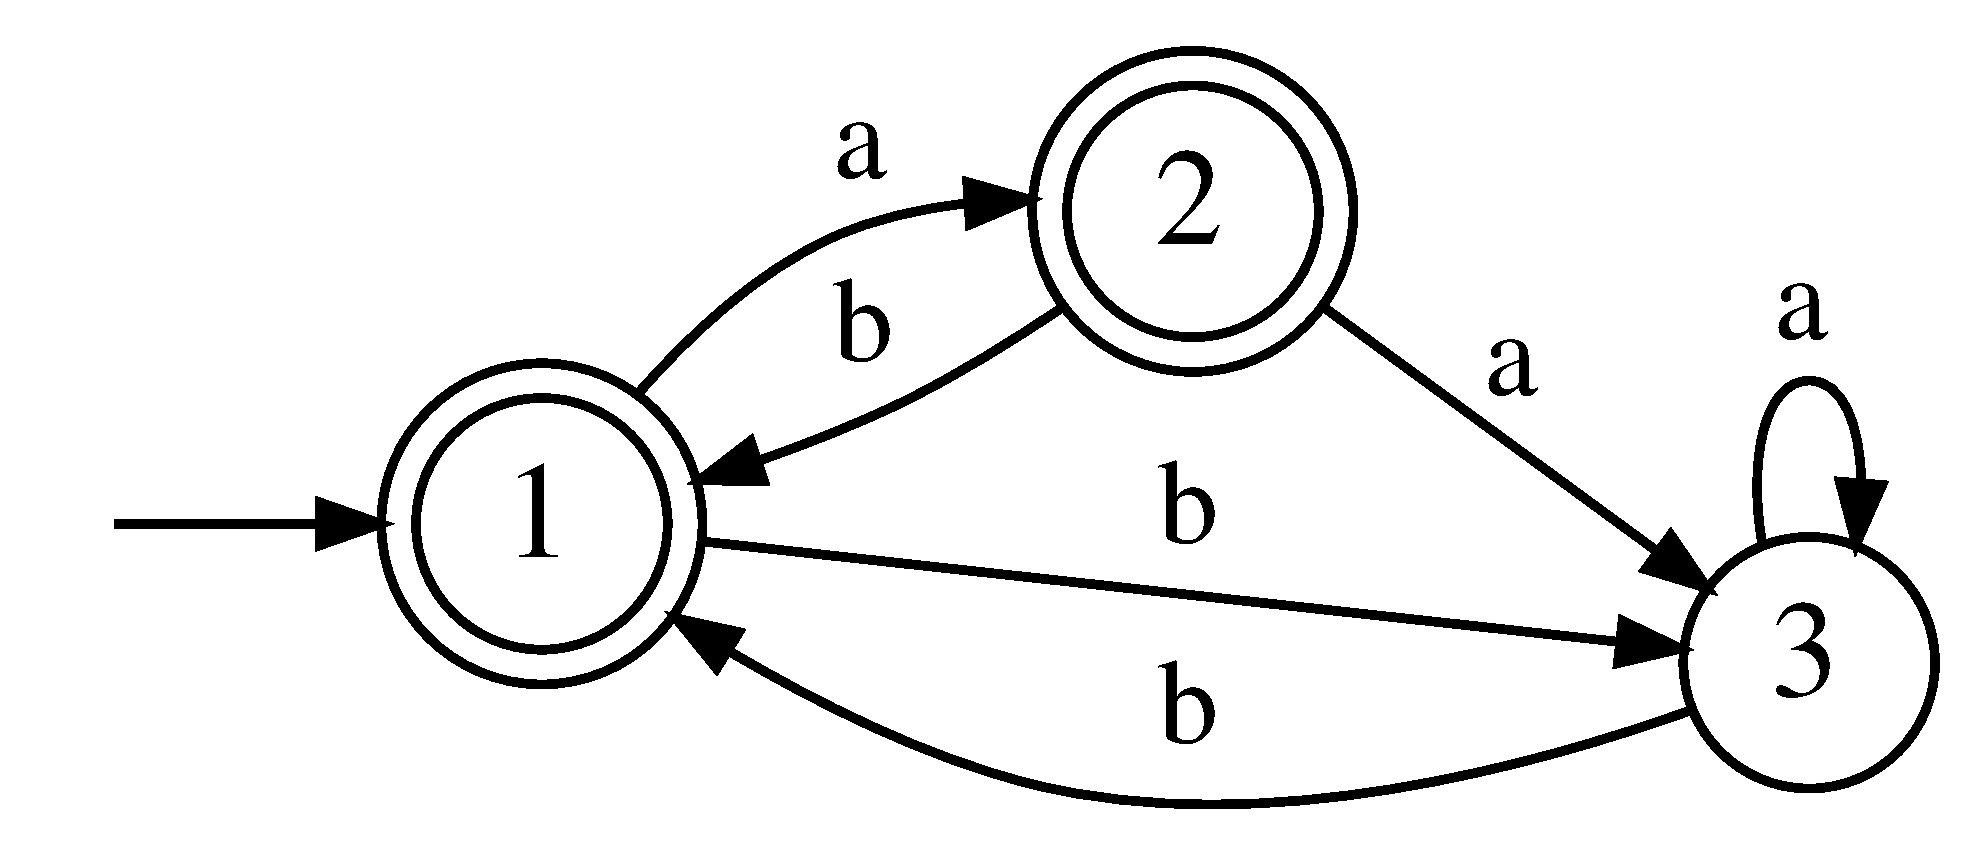
\includegraphics[scale=0.16]{img/datamod/FIG1.eps}
    \begin{tikzpicture}[
    ->, % makes the edges directed
    >=stealth', % makes the arrow heads bold
    node distance=2.5cm, % specifies the minimum distance between two nodes. Change if necessary.
    every state/.style={thick, fill=gray!10, minimum size = 0pt}, % sets the properties for each ’state’ node
    initial text=$ $, % sets the text that appears on the start arrow
    double distance between line centers=2pt
]
  \node (a1) 
    {
      \begin{tikzpicture}
        \node[state, initial] (q1) {$1$};
        \node[state, accepting] (q2) [right of=q1] {$2$};
        \node[state] (q3) [below of=q1, xshift=2.5cm/2, yshift=0.4cm] {$3$};

        \path (q1) edge [above] node {a,b} (q2)
              (q2) edge [right] node {a} (q3)
                   edge [loop above] node {b} (q2)
              (q3) edge [left] node {a,b} (q1);
      \end{tikzpicture}
    };
  \node[right of=a1, xshift=2cm] (a2)
    {
    \begin{tikzpicture}
      \node[state, initial] (q1) {$1$};
      \node[state, accepting] (q2) [right of=q1] {$3$};
      \node[state] (q3) [below of=q1, xshift=2.5cm/2, yshift=0.4cm] {$2$};

      \path (q1) edge [above] node {a,b} (q2)
            (q2) edge [right] node {a} (q3)
                 edge [loop above] node {b} (q2)
            (q3) edge [left] node {a,b} (q1);
    \end{tikzpicture}           
    };
\end{tikzpicture}
  \else
    \begin{tikzpicture}[
    ->, % makes the edges directed
    >=stealth', % makes the arrow heads bold
    node distance=1.9cm, % specifies the minimum distance between two nodes. Change if necessary.
    every state/.style={thick, fill=gray!10, minimum size = 0pt}, % sets the properties for each ’state’ node
    initial text=$ $, % sets the text that appears on the start arrow
]
  \node (a1) 
    {
      \begin{tikzpicture}
        \node[state, initial] (q1) {$1$};
        \node[state, accepting] (q2) [right of=q1] {$2$};
        \node[state] (q3) [below of=q1, xshift=1.9cm/2, yshift=0.3cm] {$3$};

        \path (q1) edge [above] node {a,b} (q2)
              (q2) edge [right] node {a} (q3)
                   edge [loop above] node {b} (q2)
              (q3) edge [left] node {a,b} (q1);
      \end{tikzpicture}
    };
  \node[right of=a1] (a2)
    {
      \node[state, initial] (q1) {$1$};
      \node[state, accepting] (q2) [right of=q1] {$3$};
      \node[state] (q3) [below of=q1, xshift=1.9cm/2, yshift=0.3cm] {$2$};

      \path (q1) edge [above] node {a,b} (q2)
            (q2) edge [right] node {a} (q3)
                 edge [loop above] node {b} (q2)
            (q3) edge [left] node {a,b} (q1);
    };
\end{tikzpicture}
  \fi
  \caption{Пример изомофрных ДКА}
  \label{img:iso-ex}
\end{figure}

\subsection{Задача генерации детерминированных конечных автоматов по заданным примерам поведения}
\label{sec:review:dfa-inf:task}

В настоящей диссертации рассматривается задача пассивного построения ДКА по имеющимся примерам поведения~\cite{DBLP:journals/pr/BugalhoO05,DBLP:journals/pr/Higuera05}~--- обучающему множеству строк, которые были приняты или отвергнуты некоторым неизвестным ДКА $\mathcal{U} = \left(U,\Sigma,\mu,u_{1},U^{+},U^{-}\right)$. 
Альтернативой является задача активного построения минимального ДКА~\cite{Angluin-active-87,DBLP:conf/sfm/SteffenHM11,neider-phd-14}, когда алгоритм построения может делать некоторые запросы к оракулу, который имеет информацию о неизвестном ДКА.

Для простоты будем считать, что примеры поведения представлены двумя множествами слов над алфавитом $\Sigma$: $S_{+}$~--- множество слов, допущенных неизвестным автоматом $\mathcal{U}$; $S_{-}$~--- множество слов, отвергнутых неизвестным автоматом $\mathcal{U}$.
Тогда задача генерации детерминированного конечного автомата заключается в поиске такого автомата, который будет принимать все слова из $S_{+}$ и отвергать все слова из $S_{-}$.
Несмотря на то, что генерация любого ДКА по заданным примерам поведения может быть решена за линейное время, задача генерации ДКА минимального размера (с минимальным числом состояний) является NP-полной~\cite{DBLP:journals/iandc/Gold78}.
Задача генерации ДКА является одной из многих задач обобщения знаний~\cite{banich2011generalization}~--- по конечному набору примеров поведения строится автомат, определяющий язык с бесконечным (хоть и счетным) числом слов.
Тогда, чем меньше автомат~--- тем лучше он описывает имеющиеся данные.
Итак, \emph{задача генерации детерминированного конечного автомата по заданным примерам поведения} заключается в поиске ДКА минимального размера, соответствующего примерам поведения.
На рисунке~\ref{img:dfa-ex} приведен пример ДКА минимального размера, построенного по множества примеров поведения $S_{+} = \{aba, bb, bba\}$ и $S_{-} = \{b, ba\}$. 

\begin{figure}[ht]
  \centering
  \ifafour
    % 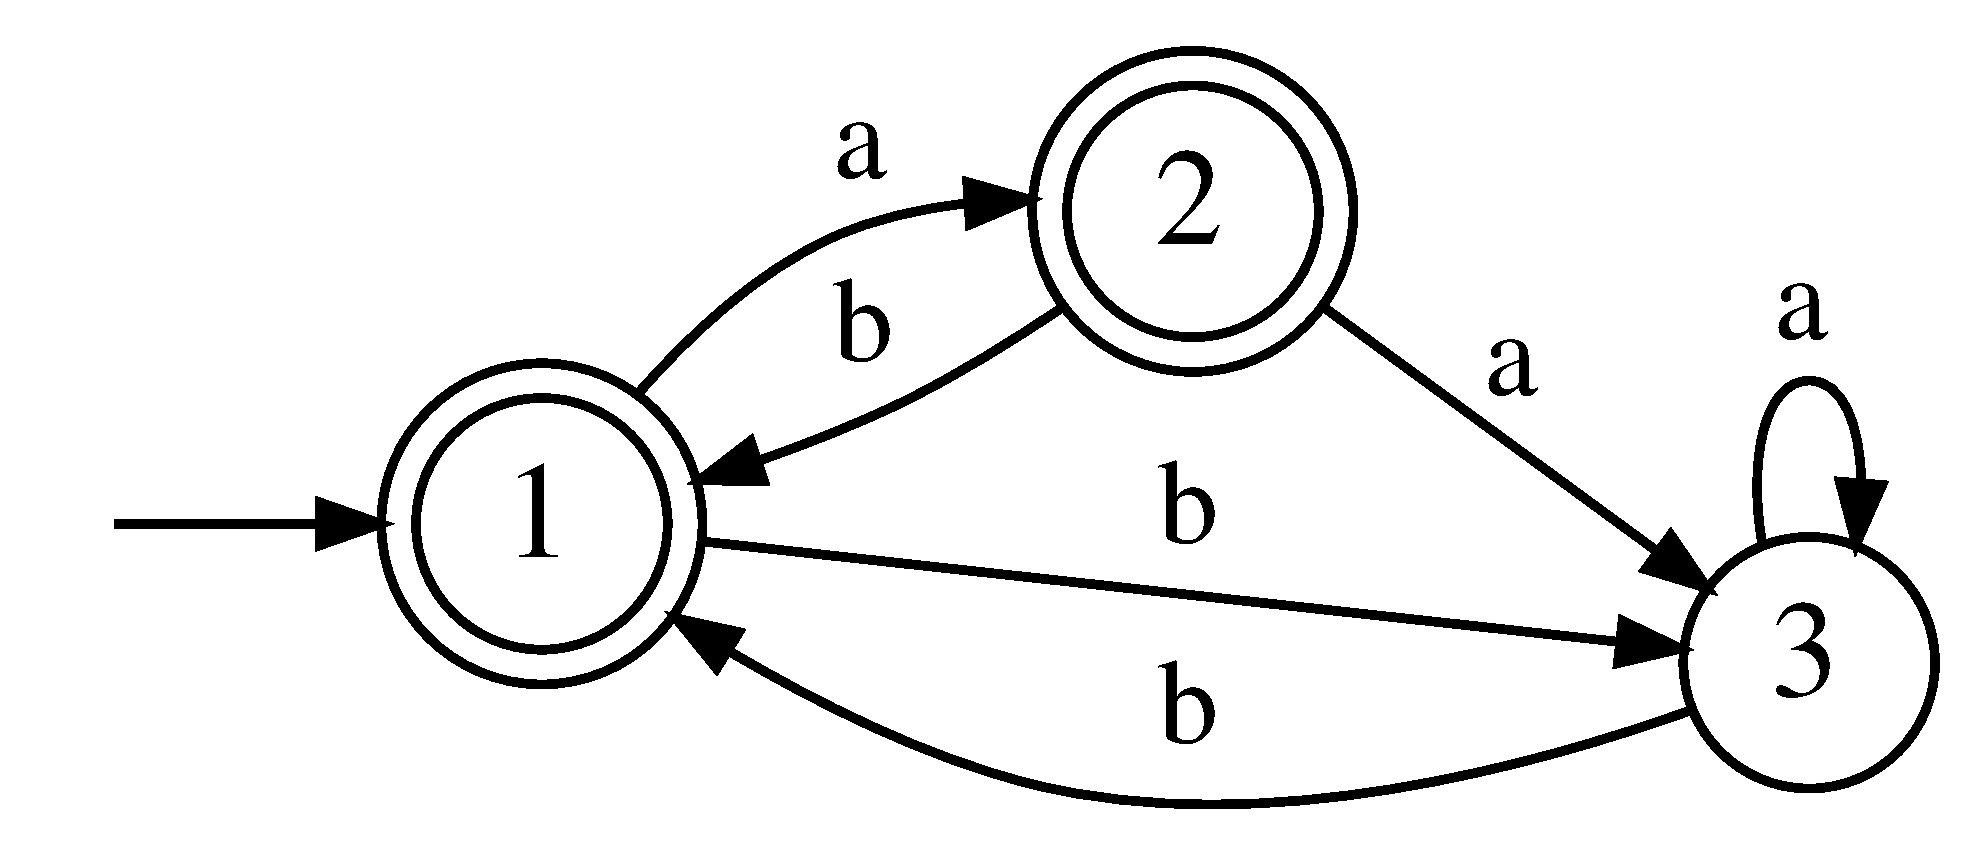
\includegraphics[scale=0.16]{img/datamod/FIG1.eps}
    \begin{tikzpicture}[
    ->, % makes the edges directed
    >=stealth', % makes the arrow heads bold
    node distance=2.5cm, % specifies the minimum distance between two nodes. Change if necessary.
    every state/.style={thick, fill=gray!10, minimum size = 0pt}, % sets the properties for each ’state’ node
    initial text=$ $, % sets the text that appears on the start arrow
    double distance between line centers=2pt
]
    \node[state, initial, accepting] (q1) {$1$};
    \node[state, accepting] (q2) [above of=q1, xshift=2.5cm/2, yshift=-0.4cm] {$2$};
    \node[state] (q3) [right of=q1] {$3$};

    \path
        (q1) edge [bend right=10, below] node [xshift=2pt] {a} (q2)
        (q2) edge [bend right=10, above] node [xshift=-2pt] {b} (q1)
        (q1) edge [bend right=10, below] node {b} (q3)
        (q3) edge [bend right=10, above] node [xshift=2pt] {b} (q1)
        (q2) edge [above] node [xshift=2pt] {a} (q3)
        (q3) edge [loop above] node {a} (q3)
        ;
\end{tikzpicture}
  \else
    \begin{tikzpicture}[
    ->, % makes the edges directed
    >=stealth', % makes the arrow heads bold
    node distance=1.9cm, % specifies the minimum distance between two nodes. Change if necessary.
    every state/.style={thick, fill=gray!10, minimum size = 0pt}, % sets the properties for each ’state’ node
    initial text=$ $, % sets the text that appears on the start arrow
]
    \node[state, initial, accepting] (q1) {$1$};
    \node[state, accepting] (q2) [above of=q1, xshift=1.9cm/2, yshift=-0.3cm] {$2$};
    \node[state] (q3) [right of=q1] {$3$};

    \path
        (q1) edge [bend right=10, below] node [xshift=2pt] {a} (q2)
        (q2) edge [bend right=10, above] node [xshift=-2pt] {b} (q1)
        (q1) edge [bend right=10, below] node {b} (q3)
        (q3) edge [bend right=10, above] node {b} (q1)
        (q2) edge [above] node [xshift=2pt] {a} (q3)
        (q3) edge [loop above] node {a} (q3)
        ;
\end{tikzpicture}
  \fi
  \caption{Пример ДКА минимального размера, соответствующего наборам примеров поведения $S_{+} = \{aba, bb, bba\}$ и $S_{-} = \{b, ba\}$}
  \label{img:dfa-ex}
\end{figure}

\subsection{Расширенное префиксное дерево}
\label{sec:review:dfa-inf:apta}

Первым шагом большинства существующих подходов является построение \emph{расширенного префиксного дерева} (augmented prefix tree acceptor~{---} APTA) по имеющимся множествам примеров поведения $S_{+}$ и $S_{-}$. 
Расширенное префиксное дерево~--- это древовидная структура данных, основанная на обычном префиксном дереве (бор, нагруженное дерево, prefix tree, trie), отличающаяся от нее метками вершин.
Более формально, префиксным деревом называется шестерка $\mathcal{T} = \left(T,\Sigma,\tau,t_{1},T^{+}, T^{-}\right)$, где $T$~{---} конечное множество вершин, $\Sigma$~{---} алфавит входных символов, $\tau: T \times \Sigma \pto T$~{---} \emph{функция переходов}, $t_{1}$~{---} \emph{корневая} вершина (\emph{корень}), $T^{+} \subset T$~{---} множество \emph{допускающих} (\emph{принимающих}) вершин, $T^{-} \subset T$~{---} множество \emph{не допускающих} (\emph{отвергающих}) вершин.
В отличие от функции переходов в ДКА, функция переходов $\tau$ является частичной. 
Также, в префиксном дереве $T^{+} \cup T^{-} \subset T$, то есть некоторые вершины могут не являться ни принимающими, ни отвергающими~--- промежуточные вершины.

Расширенное префиксное дерево для множеств примеров поведения $S_{+}$ и $S_{-}$ строится как обычное префиксное дерево, но терминальные вершины для каждого слова помечаются соответствующей меткой. Вершины, в которых не заканчивается ни один из примеров поведения, остаются непомеченными. Пример расширенного префиксного дерева приведен на рисунку~\ref{img:apta-ex}.
Также далее в диссертации с помощью $\Delta(v)$ будет обозначаться расстояния от корневой вершины $t_{1}$ до вершины $t_{v}$.

\begin{figure}[ht]
  \centering
  \ifafour
    % 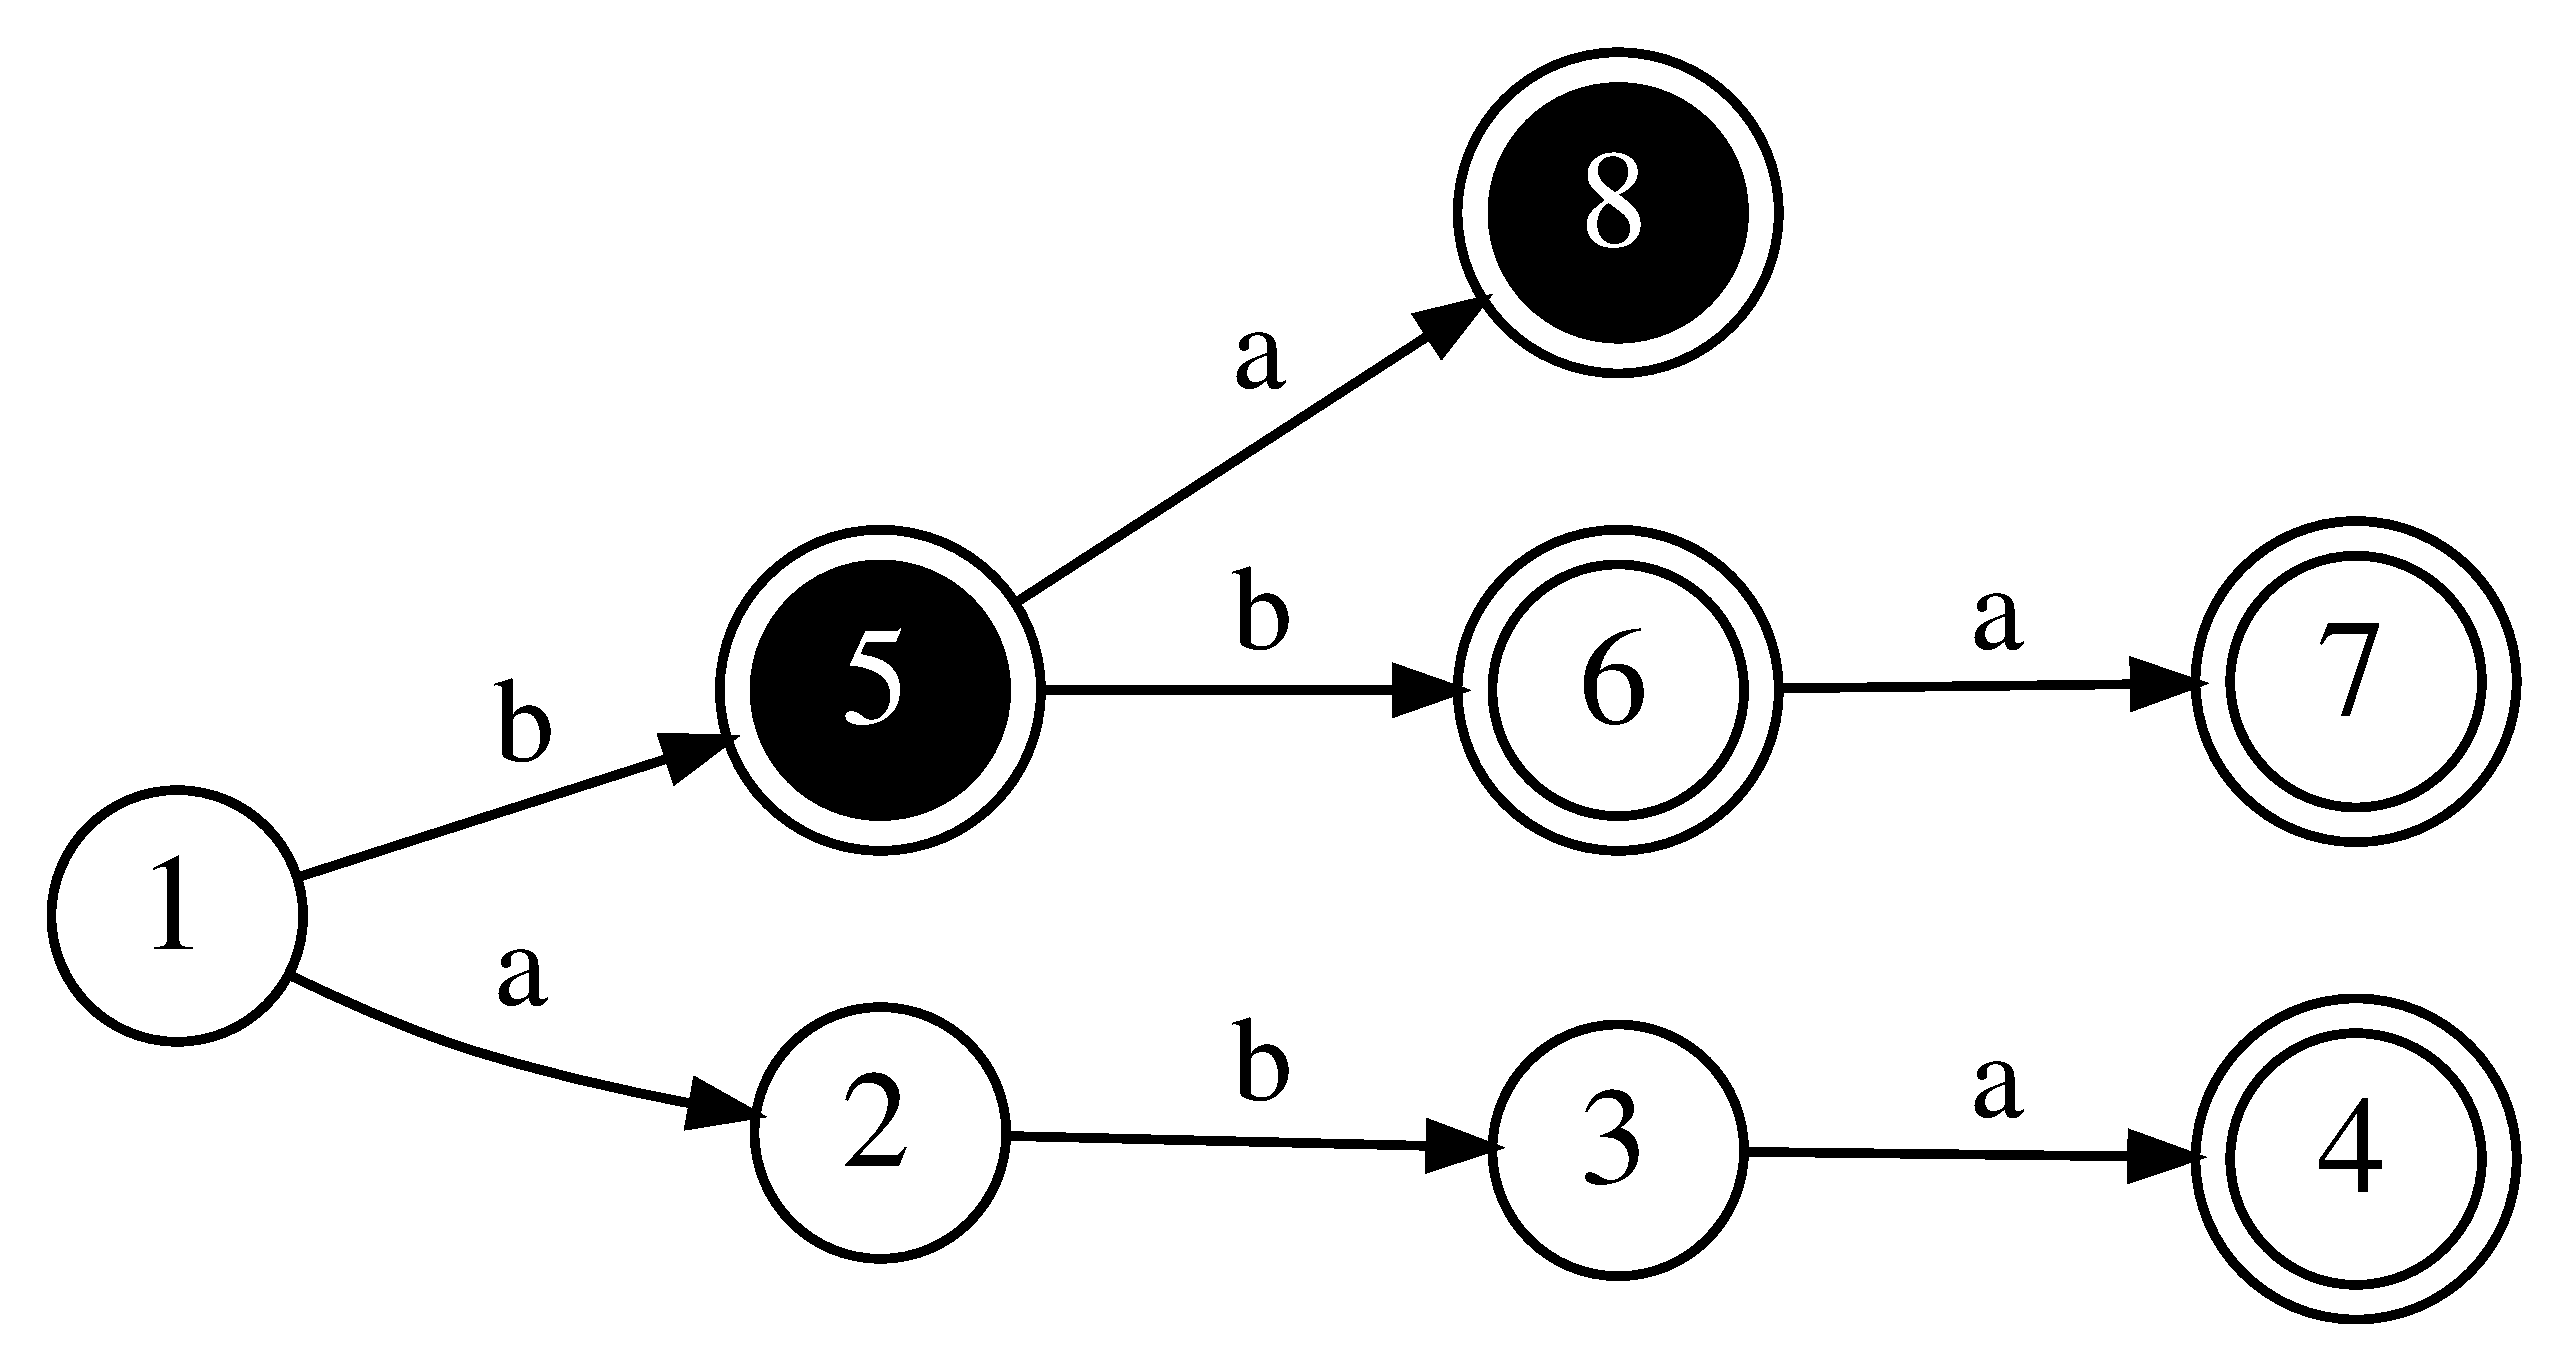
\includegraphics[scale=0.14]{img/datamod/FIG2a.eps}
    \begin{tikzpicture}[
    ->, % makes the edges directed
    >=stealth', % makes the arrow heads bold
    node distance=2cm, % specifies the minimum distance between two nodes. Change if necessary.
    every state/.style={thick, fill=gray!10, minimum size = 0pt}, % sets the properties for each ’state’ node
    initial text=$ $, % sets the text that appears on the start arrow
    double distance between line centers=2pt
]
    \def\yshift{0.47cm}
    \def\xshift{0.26cm}

    \node[state, initial] (q1) {$1$};
    \node[state, fill=white, dashed, inner sep=9.7pt] (q5) [above right of=q1, yshift=-\yshift, xshift=\xshift] {};
    \node[state, inner sep=4.2pt] (dummy5) [above right of=q1, yshift=-\yshift, xshift=\xshift] {$5$};
    \node[state, accepting] (q6) [right of=q5] {$6$};
    \node[state, accepting] (q7) [right of=q6] {$7$};
    \node[state] (q2) [below right of=q1, yshift=\yshift, xshift=\xshift] {$2$};
    \node[state] (q3) [right of=q2] {$3$};
    \node[state, accepting] (q4) [right of=q3] {$4$};
    \node[state, fill=white, dashed, inner sep=9.7pt] (q8) [above of=q6, yshift=-0.78cm] {};
    \node[state, inner sep=4.2pt] (dummy8) [above of=q6, yshift=-0.78cm] {$8$};

    \path 
        (q1) edge [above] node {b} (q5)
        (q5) edge [below] node {b} (q6)
        (q6) edge [below] node {a} (q7)
        (q5) edge [above] node {a} (q8)
        (q1) edge [below] node {a} (q2)
        (q2) edge [below] node {b} (q3)
        (q3) edge [below] node {a} (q4)
        ;
\end{tikzpicture}
  \else
    \begin{tikzpicture}[
    ->, % makes the edges directed
    >=stealth', % makes the arrow heads bold
    node distance=1.5cm, % specifies the minimum distance between two nodes. Change if necessary.
    every state/.style={thick, fill=gray!10, minimum size = 0pt}, % sets the properties for each ’state’ node
    initial text=$ $, % sets the text that appears on the start arrow
]
    \def\yshift{0.36cm}
    \def\xshift{0.2cm}

    \node[state, initial] (q1) {$1$};
    \node[state, dashed, inner sep=7pt] (q5) [above right of=q1, yshift=-\yshift, xshift=\xshift] {};
    \node[state, inner sep=3pt] (dummy5) [above right of=q1, yshift=-\yshift, xshift=\xshift] {$5$};
    \node[state, accepting] (q6) [right of=q5] {$6$};
    \node[state, accepting] (q7) [right of=q6] {$7$};
    \node[state] (q2) [below right of=q1, yshift=\yshift, xshift=\xshift] {$2$};
    \node[state] (q3) [right of=q2] {$3$};
    \node[state, accepting] (q4) [right of=q3] {$4$};
    \node[state, dashed, inner sep=7pt] (q8) [above of=q6, yshift=-0.58cm] {};
    \node[state, inner sep=3pt] (dummy8) [above of=q6, yshift=-0.58cm] {$8$};

    \path 
        (q1) edge [above] node {b} (q5)
        (q5) edge [below] node {b} (q6)
        (q6) edge [below] node {a} (q7)
        (q5) edge [above] node {a} (q8)
        (q1) edge [below] node {a} (q2)
        (q2) edge [below] node {b} (q3)
        (q3) edge [below] node {a} (q4)
        ;
\end{tikzpicture}
  \fi
  \caption{Пример расширенного префиксного дерева, построенного по наборам примеров поведения $S_{+} = \{aba, bb, bba\}$ и $S_{-} = \{b, ba\}$}
  \label{img:apta-ex}
\end{figure}

%----------------------------------------------------------------------------------------

\section{Эвристические и метаэвристические методы генерации детерминированных конечных автоматов} 
\label{sec:review:heuristic-dfa-inf}

В настоящем разделе приводится обзор существующих эвристических и метаэвристических методов генерации ДКА минимального размера по заданным примерам поведения.
Отличительной особенностью таких методов является то, что они не являются точными~--- ими не гарантируется, что какой-то ДКА будет найден в принципе, а если ДКА найден, то не гарантируется его минимальность.
Несмотря на то, что настоящая диссертация посвящена расширению границ применимости точных методов генерации ДКА, для построения достаточно больших автоматов по большому числу примеров поведения неточные эвристические и метаэвристические методы все еще являются единственным возможным вариантом.

\paragraph*{Эвристические алгоритмы.}
\label{sec:review:heuristic-dfa-inf:heuristic}
В основе эвристических алгоритмов лежит идея \emph{слияния состояний} (\emph{state merging})~--- последовательных объединения вершин расширенного префиксного дерева и устранения образующейся недетерминированности.
Первый известный алгоритм для решения данной задачи был предложен в работе Трахтенброта и Барздиня в 1970 году~\cite{trakhtenbrot-1973-modeling}~--- \texttt{TB}-алгоритм.
Однако, предложенный алгоритм решает только частный случай задачи генерации ДКА по заданным примерам поведения: для некоторого натурального $k$ все возможные слова длины $k$ над алфавитом $\Sigma$~--- всего $\abs{\Sigma}^{k}$ слов~--- должны содержаться во множествах $S_{+}$ и $S_{-}$.
\texttt{TB}-алгоритм основан на полном переборе всех возможных пар состояний префиксного дерева и слиянии эквивалентных состояний в одно.

В 1978 году Голд доказал NP-полноту задачи генерации ДКА заданного, а значит и минимального, размера~\cite{DBLP:journals/iandc/Gold78}.
Ввиду указанной сложности новые алгоритмы генерации минимального ДКА не предлагались более десяти лет.
В последующие годы разрабатывались исключительно неточные эвристические алгоритмы.
Среди таких алгоритмов можно выделить следующие: \texttt{traxbar}~\cite{DBLP:conf/colt/Lang92}, \texttt{RPNI}~\cite{oncina-rpni-1992}, \texttt{EDSM}~\cite{DBLP:conf/icgi/LangPP98}, \texttt{exbar}~\cite{lang-1999-faster}, \texttt{Windowed-EDSM}~\cite{DBLP:conf/icgi/CicchelloK02}.
Все перечисленные алгоритмы основаны на слиянии состояний расширенного префиксного дерева.
Состояния для слияния выбираются эвристически, чем одновременно объясняется высокая скорость работы и неточность данных алгоритмов.

Самым успешным среди перечисленных эвристических алгоритмов можно считать алгоритм \emph{объединения состояний на основе свидетельств} (\emph{evidence-driven state merging}~--- EDSM)~\cite{DBLP:conf/icgi/LangPP98}.
На каждой итерации алгоритм EDSM хранит текущую версию частично построенного ДКА.
Изначально в качество такого ДКА выступает расширенное префиксное дерево.
Затем на каждом шаге эвристически осуществляется выбор двух состояний текущего частично построенного ДКА, которые \emph{объединяются} (\emph{сливаются}) в одно состояние.
При слиянии двух состояний может возникнуть недетерминированность~--- несколько исходящих переходов из нового состояния, помеченных одним и тем же символом.
Недетерминированность устраняется с помощью рекурсивного слияния тех состояний, в которые ведут переходы с одинаковыми метками.
Данный процесс повторяется до тех пор, пока существуют пары состояний, пригодные для слияния. 
Нетривиальным шагом является выбор состояний для объединения.
Ситуация, когда происходит объединение принимающего и отвергающего состояния называется \emph{конфликтом}.
Для построения корректного ДКА не могут проводиться слияния, приводящие к конфликтам.
Состояния, одно из которых помечено как принимающее, а другое~--- как отвергающее, не могут быть объединены в одно состояние, так как это незамедлительно приводит к конфликту.
Если объединение двух состояний не приводит незамедлительно к конфликту (сливаются два принимающих состояния, два отвергающих состояния, либо одно из состояний является неопределенным), то конфликт может возникнуть при дальнейшем устранении недетерминированности.
Перебор всех возможных пар состояний занимает экспоненциальное время, поэтому и используются эвристики для выбора подходящих пар.
В основе алгоритма EDSM лежит эвристика выбора состояний для слияния, основанная на подсчете различных характеристик на поддеревьях потенциальных кандидатов для объединения.
Например, может подсчитываться число исходящих переходов из каждого состояния по одним и тем же символам.
Таким образом, жадно выбираются пары состояний имеющие максимальное значение соответствующих характеристик и происходит процесс слияния и устранения недетерминированности.
Первые слияния состояний близких к корню расширенного префиксного дерева с большой вероятностью не увеличивают размер итогового автомата в виду большого размера поддеревьев и высоких показателей оценочных характеристик.
Однако, чем ближе к листьям дерева, тем меньше поддеревья и тем меньше точность таких слияний.
Данный алгоритм демонстрирует высокую скорость работы, однако генерируемый ДКА зачастую значительно больше, чем минимально возможный, соответствующий заданным примерам поведения.
Алгоритм EDSM является победителем соревнования \emph{Abbadingo One DFA Learning Competition}~\cite{DBLP:conf/icgi/LangPP98}, посвященному генерации ДКА.

\paragraph*{Метаэвристические алгоритмы.}
\label{sec:review:heuristic-dfa-inf:metaheuristic}
Среди метаэвристических алгоритмов, успешно применяемых для генерации конечных автоматов по примерам поведения, можно выделить эволюционные стратегии, генетические алгоритмы и муравьиные алгоритмы.

Эволюционные алгоритмы получили свое название в честь эволюционной теории Дарвина, упрощенная версия которой и лежит в их основе.
Эволюционные стратегии и генетические алгоритмы являются разновидностями эволюционных алгоритмов.
В эволюционных стратегиях обычно используются только оператор мутации, в то время как в генетических алгоритмах используются как оператор мутации, так и оператор скрещивания.
В ходе своей работы такие алгоритмы поддерживают популяцию особей~--- в данном случае различных детерминированных конечных автоматов,~--- являющихся кандидатами на решение исходной задачи.
Изначально автоматы выбираются случайным образом, а затем при помощи операторов мутации и скрещивания генерируются новые автоматы.
На каждой итерации для каждого из полученных автоматов рассчитывается функция приспособленности, оценивающая насколько хорошо текущий автомат описывает заданные примеры поведения.
Затем, лучшие из особей остаются в популяции, а худшие исключаются из рассмотрения.
С помощью операторов мутации, меняющего незначительно одиночный автомат, и скрещивания, определенным образом объединяющих два автомата, генерируется новые особи на замену исключенным.
Такой процесс повторяется, пока не будет найден автомат, достаточно хорошо описывающий примеры поведения, либо пока не выйдет заданное время.
Среди эволюционных стратегий для генерации ДКА можно выделить алгоритмы, описанные в работе Лукаса и Рейнольдса~\cite{DBLP:journals/pami/LucasR05} и в работе Гомеза~\cite{DBLP:conf/cec/Gomez06}.
Среди генетических алгоритмов можно выделить алгоритм, предложенный в Университете ИТМО ученым Егоровым,~\cite{genetic-algs-dfa-inf-egorov-13}.

В работе Чивилихина~\cite{chivilikhin-phd-15}, выполненной в Университете ИТМО, был предложен метод \texttt{MuACO} для генерации конечных автоматов по заданной функции приспособленности.
В основе данного метода используются идеи муравьиных алгоритмов оптимизации~\cite{DBLP:reference/ml/DorigoB17}.
Муравьиные алгоритмы~--- это класс метаэвристик, предназначенных для решения оптимизационных задач.
В основе данных алгоритмов лежит биологический процесс поиска пищи у муравьев.
В методе \texttt{MuACO} используется такая структура данных, как граф мутаций.
Вершинами данного графа являются конечные автоматы, потенциально являющиеся решением задачи генерации ДКА по заданным примерам поведения, а ребрам соответствуют мутации автоматов~--- небольшие изменения в структуре переходов автомата или во множестве допускающих состояний автомата.
Каждому ребру в графе мутации соответствует некоторое значение эвристической информации и феромона.
Эвристическая информация и феромон являются некоторыми вспомогательными величинами, используемыми при генерации новых автоматов.
Каждый шаг алгоритма представляется в виде движения виртуальных муравьев по графу мутаций.
Периодически значения эвристической информации и феромона обновляется в зависимости от того, насколько текущий автомат хорошо описывает заданные примеры поведения.
Такой процесс также повторяется, пока не будет найден автомат, достаточно хорошо описывающий примеры поведения, либо пока не выйдет заданное время.

Метаэвристические алгоритмы также являются неточными~--- ими вообще не гарантируется, что какое-то решение будет найдено за конечное время, поэтому сравнение с ними в настоящей диссертации, направленной на развитие точных методов генерации ДКА, не проводилось.

%----------------------------------------------------------------------------------------

\section{Методы генерации детерминированных конечных автоматов, основанные на сведении к другим NP-трудным задачам} 
\label{sec:review:sat-dfa-inf} 

В настоящем разделе приводится обзор существующих точных методов генерации ДКА по заданным примерам поведения при помощи сведений к задачам раскраски графа и выполнимости булевой формулы.
Также приводится обзор существующих подходов к нарушению симметрии.

Лучшие эвристики выбора пары состояний для слияния в алгоритме EDSM обычно основаны на успешных эвристиках для других гораздо более активно изучаемых задач, например, для задачи выполнимости или задачи раскраски графа.
Как уже говорилось, ежегодно проходят соревнования по определению лучшего программного средства для решения SAT~\cite{sat-competitions}.
Несмотря на то, что различные эвристические стратегии выбора вершин для слияния повышают производительность метода EDSM и при его реализации используются оптимизированные структуры данных, данные реализации все еще значительно проигрывают по эффективности программным средствам для решения более проработанных задач.
Так как задача генерации ДКА является NP-полной~\cite{DBLP:journals/iandc/Gold78}, то ее можно свести к задачам, которые изучаются дольше и интенсивнее, чтобы использовать максимально оптимизированные стратегии поиска решения.

\subsection{Метод, основанный на сведении к задаче раскраски графа}
\label{sec:review:sat-dfa-inf:coloring}

В работе французских ученых Косте и Николя~\cite{Coste97regularinference} предлагается сведение задачи генерации ДКА по заданным примерам поведения к задаче раскраски графа.
На первом шаге алгоритма как и ранее строится расширенное префиксное дерево по заданным примерам поведения.
Основной идей предложенного сведения является использование различных цветов для каждого из состояний генерируемого ДКА.
Раскраска производится таким образом, что, если все вершины расширенного префиксного дерева, соответствующие одному цвету в раскрашиваемом графе, объединить в одно состояние автомата, и проделать данную операцию для всех цветов, то в итоге должен получиться детерминированный конечный автомат. 

Ситуация, когда объединяются допускающая и отвергающая вершины графа, называется \emph{конфликтом}, так как состояние ДКА может быть только либо допускающим, либо отвергающим.
Очевидно, что тогда две вершины соединены ребром, если одна из них помечена как допускающая, а другая как отвергающая, так как их объединение приводит к конфликту.
Использование расширенного префиксного дерева, в котором существуют вершины, помеченные как промежуточные (то есть не являющиеся ни принимающими, ни отвергающими), позволяет в явном виде находить некоторые конфликты, которые возникают при объединении двух вершин, одна или две из которых являются промежуточными.
Объединение двух вершин расширенного префиксного дерева в одну может привести к недетерминированности~--- для новой вершины будет существовать несколько исходящих переходов, помеченных одним символом.
Избавиться от недетерминированности можно с помощью детерминизации~--- рекурсивного объединив вершины, куда ведут такие переходы.
Если в процессе детерминизации возникает конфликт, то можно утверждать, что слияние вершин, объединенных на каждом из предыдущих шагов, приводит к конфликту.

Тогда, отметив в графе все найденные конфликты, можно перейти к решению задачи раскраски графа в $k$ цветов.
Так как исходная задача заключается в поиске ДКА с минимальным числом состояний, то требуется найти минимальное $k$ для которого существует правильная раскраска.
Добиться этого предлагается путем итеративного перебора числа цветов $k$, начиная с единицы и до тех пор, пока не будет найдено решение.
На рисунке~\ref{img:apta-color} представлен пример расширенного префиксного дерева, раскрашенного в три цвета так, что для каждого цвета объединение всех вершин данного цвета в одно состояние не приводит к несовместимости.

\begin{figure}[ht]
  \centering
  \ifafour
    \begin{tikzpicture}[
    ->, % makes the edges directed
    >=stealth', % makes the arrow heads bold
    node distance=2cm, % specifies the minimum distance between two nodes. Change if necessary.
    every state/.style={thick, fill=gray!10, minimum size = 0pt}, % sets the properties for each ’state’ node
    initial text=$ $, % sets the text that appears on the start arrow
    double distance between line centers=2pt
]
    \def\yshift{0.47cm}
    \def\xshift{0.26cm}
    
    \def\lightred{red!40}
    \def\lightblue{blue!30}
    \def\lightyellow{yellow!70}

    \node[state, initial, fill=\lightred] (q1) {$1$};
    \node[state, accepting, fill=\lightyellow] (q2) [above right of=q1, yshift=-\yshift, xshift=\xshift] {$2$};
    \node[state, fill=\lightyellow] (q3) [below right of=q1, yshift=\yshift, xshift=\xshift] {$3$};
    \node[state, fill=white, dashed, inner sep=9.7pt] (q5) [right of=q2] {};
    \node[state, fill=\lightblue, inner sep=4.2pt] (dummy5) [right of=q2] {$5$};
    \node[state, fill=\lightblue] (q8) [right of=q3] {$8$};
    \node[state, fill=\lightred] (q6) [right of=q5] {$6$};
    \node[state, fill=white, dashed, inner sep=9.7pt] (q9) [right of=q8] {};
    \node[state, fill=\lightred, inner sep=4.2pt] (dummy9) [right of=q8] {$9$};
    \node[state, accepting, fill=\lightyellow] (q7) [right of=q6] {$7$};
    \node[state, accepting, fill=\lightyellow] (q4) [below of=q8, yshift=0.78cm] {$4$};

    \path 
        (q1) edge [above] node {a} (q2)
        (q2) edge [above] node {a} (q5)
        (q5) edge [above] node {a} (q6)
        (q6) edge [above] node {a} (q7)
        (q1) edge [above] node {b} (q3)
        (q3) edge [above] node {a} (q8)
        (q8) edge [above] node {b} (q9)
        (q3) edge [below] node {b} (q4)
        ;
\end{tikzpicture}
  \else
    \begin{tikzpicture}[
    ->, % makes the edges directed
    >=stealth', % makes the arrow heads bold
    node distance=2.5cm, % specifies the minimum distance between two nodes. Change if necessary.
    every state/.style={thick, fill=gray!10}, % sets the properties for each ’state’ node
    initial text=$ $, % sets the text that appears on the start arrow
]
    \def\yshift{0.36cm}
    \def\xshift{0.2cm}
    
    \def\lightred{red!40}
    \def\lightblue{blue!30}
    \def\lightyellow{yellow!70}

    \node[state, initial, fill=\lightred] (q1) {$1$};
    \node[state, accepting, fill=\lightyellow] (q2) [above right of=q1, yshift=-\yshift, xshift=\xshift] {$2$};
    \node[state, fill=\lightyellow] (q3) [below right of=q1, yshift=\yshift, xshift=\xshift] {$3$};
    \node[state, fill=white, dashed, inner sep=9pt] (q5) [right of=q2] {};
    \node[state, fill=\lightblue, inner sep=4pt] (dummy5) [right of=q2] {$5$};
    \node[state, fill=\lightblue] (q8) [right of=q3] {$8$};
    \node[state, fill=\lightred] (q6) [right of=q5] {$6$};
    \node[state, fill=white, dashed, inner sep=9pt] (q9) [right of=q8] {};
    \node[state, fill=\lightred, inner sep=4pt] (dummy9) [right of=q8] {$9$};
    \node[state, accepting, fill=\lightyellow] (q7) [right of=q6] {$7$};
    \node[state, accepting, fill=\lightyellow] (q4) [below of=q8, yshift=0.58cm] {$4$};

    \path 
        (q1) edge [above] node {a} (q2)
        (q2) edge [above] node {a} (q5)
        (q5) edge [above] node {a} (q6)
        (q6) edge [above] node {a} (q7)
        (q1) edge [above] node {b} (q3)
        (q3) edge [above] node {a} (q8)
        (q8) edge [above] node {b} (q9)
        (q3) edge [below] node {b} (q4)
        ;
\end{tikzpicture}
  \fi
  \caption{Пример расширенного префиксного дерева, построенного по множествам примеров поведения $S_{+}=\{a;aaaa;bb\}$ и $S_{-}=\{aa;bab\}$ и раскрашенного в три цвета так, что для каждого цвета объединение всех вершин данного цвета в одно состояние не приводит к несовместимости}
  \label{img:apta-color}
\end{figure}

На рисунке~\ref{img:dfa-color} представлен пример ДКА, построенного путем объединения вершин расширенного префиксного дерева, изображенного на рисунке~\ref{img:apta-color}, покрашенных в один цвет в одно состояние автомата.

\begin{figure}[ht]
  \centering
  \ifafour
    \begin{tikzpicture}[
    ->, % makes the edges directed
    >=stealth', % makes the arrow heads bold
    node distance=2.5cm, % specifies the minimum distance between two nodes. Change if necessary.
    every state/.style={thick, fill=gray!10, minimum size = 0pt}, % sets the properties for each ’state’ node
    initial text=$ $, % sets the text that appears on the start arrow
    double distance between line centers=2pt
]
    \def\lightred{red!40}
    \def\lightblue{blue!30}
    \def\lightyellow{yellow!70}

    \node[state, initial, fill=\lightred] (q1) {$1$};
    \node[state, accepting, fill=\lightyellow] (q2) [right of=q1] {$2$};
    \node[state,fill=\lightblue] (q3) [below of=q1, xshift=2.5cm/2, yshift=0.4cm] {$3$};

    \path 
        (q1) edge [above] node {a,b} (q2)
        (q2) edge [right] node {a} (q3)
             edge [loop above] node {b} (q2)
        (q3) edge [left] node {a,b} (q1)
        ;
\end{tikzpicture}
  \else
    \begin{tikzpicture}[
    ->, % makes the edges directed
    >=stealth', % makes the arrow heads bold
    node distance=2.5cm, % specifies the minimum distance between two nodes. Change if necessary.
    every state/.style={thick, fill=gray!10}, % sets the properties for each ’state’ node
    initial text=$ $, % sets the text that appears on the start arrow
]
    \def\lightred{red!40}
    \def\lightblue{blue!30}
    \def\lightyellow{yellow!70}

    \node[state, initial, fill=\lightred] (q1) {$1$};
    \node[state, accepting, fill=\lightyellow] (q2) [right of=q1] {$2$};
    \node[state,fill=\lightblue] (q3) [below of=q1, xshift=2.5cm/2, yshift=0.3cm] {$3$};

    \path 
        (q1) edge [above] node {a,b} (q2)
        (q2) edge [right] node {a} (q3)
             edge [loop above] node {b} (q2)
        (q3) edge [left] node {a,b} (q1)
        ;
\end{tikzpicture}
  \fi
  \caption{Пример ДКА, получающегося после объединения вершин одного цвета в расширенном префиксном дереве, представленном на рисунке~\ref{img:apta-color}}
  \label{img:dfa-color}
\end{figure}

\subsection{Методы, основанные на сведении к задаче выполнимости}
\label{sec:review:sat-dfa-inf:sat}

Как было сказано в разделе~\ref{sec:review:sat:methods}, программные средства для решения задачи выполнимости в последние несколько десятилетий~--- фактически с 1996 года, когда был предложен алгоритм CDCL~--- сильно развились и стали достаточно мощными средствами для решения многих прикладных задач, выраженных на языке SAT.
Например, сведение к SAT используется для решения таких задач, как символьная проверка моделей~\cite{DBLP:conf/tacas/BiereCCZ99}, поиск связей между различными контекстами в распределенных системах~\cite{DBLP:conf/context/BouquetMSZ03}, поиск ошибок в программах на языке программирования \texttt{C}~\cite{DBLP:conf/cav/XieA05}, поиск кратчайшего синхронизирующего слова~\cite{DBLP:conf/wia/SkvortsovT11}, кластеризация в ограничения~\cite{DBLP:conf/ida/MetivierBCKL12}, генерация оптимальных деревьев решений~\cite{DBLP:conf/ijcai/NarodytskaIPM18} и множества других.

\paragraph*{DFASAT.}
В 2010 году в статье~\cite{heule-icgi10} учеными Марейном Хойлом (Marijn Heule) и Сикко Вервером (Sicco Verwer) впервые был предложен метод генерации ДКА по заданным примерам поведения, основанный на сведении к задаче выполнимости, названный DFASAT.
Метод DFASAT основан на описанном в предыдущем разделе сведении задачи генерации ДКА к задаче раскраски графа.
Метод DFASAT состоит из следующих этапов, которые будут подробнее описаны далее.
Как и ранее, первым шагом метода является построение расширенного префиксного дерева по имеющимся примерам поведения.
Затем, выбирается нижняя оценка на размера искомого автомата $M$. 
В простейшем случае, в качестве нижней оценки выбирается значение $M = 2$, если имеются как положительные, так и отрицательные примеры поведения, однако, какие-то более сложные оценки могут также использоваться.
Далее строится булева КНФ-формула, кодирующая задачу генерации ДКА текущего размера $M$, соответствующего заданным примерам поведения, представленным в виде расширенного префиксного дерева.
Построенная формула передается на вход программному средству для решения SAT, которое решает задачу выполнимости.
Если формула выполнима, то программное средство возвращает выполняющую подстановку, по которой, затем, строится ДКА, являющийся решением исходной задачи генерации ДКА минимального размера по примерам поведения.
В случае, если формула невыполнима, размер искомого автомата увеличивается на единицу и процесс повторяется заново с построения булевой КНФ-формулы.
Такой итеративный процесс повторяется до тех пор, пока для некоторого $M$ не будет найдена выполняющая выполняющая подстановка для соответствующей формулы, что гарантирует минимальность найденного автомата.
Схема метода DFASAT представлена на рисунке~\ref{img:dfasat-algo}.
%
\begin{figure}[ht]
  \centering
  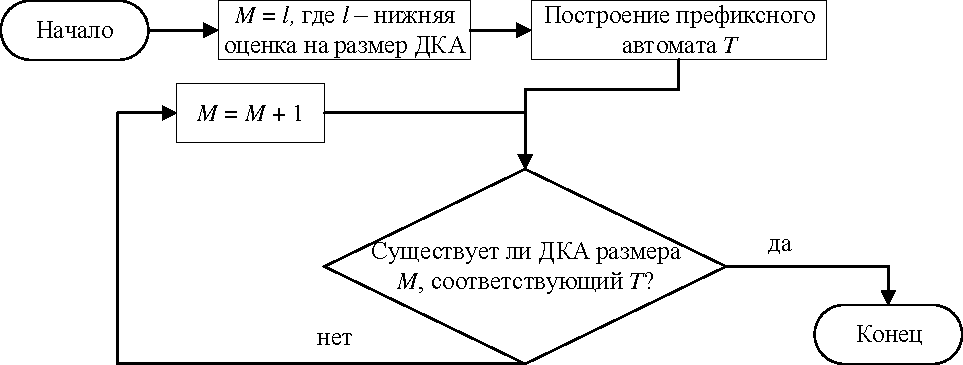
\includegraphics[scale=0.9]{img/ntv/basic.pdf}
  \caption{Схема точного метода генерации ДКА по заданным примерам поведения на основе сведения к SAT~--- \texttt{DFASAT}}
  \label{img:dfasat-algo}
\end{figure}

Построение префиксного дерева описывалось в разделе~\ref{sec:review:dfa-inf:apta}.
Следующим шагом метода DFASAT является построение булевой формулы на языке SAT.
Существует широко известное сведение задачи раскраски графа к SAT, которое Хойл и Вервер называют \emph{прямым кодированием} (\emph{direct encoding})~\cite{DBLP:conf/cp/Walsh00}.
Однако, авторы показывают, что использование прямого кодирования для задачи генерации ДКА приводит к построению булевой формулы, состоящей из $\mathcal{O}\left(N^{2} \times M^{2}\right)$, где $N$~--- размер префиксного дерева, $M$~--- размер генерируемого автомата, дизъюнктов.
Для нетривиальных примеров задачи генерации ДКА формула такого сложности получается слишком большой для современных программных средств для решения SAT, поэтому голландские ученые предложили \emph{компактное сведение} (\emph{compact encoding}).

Здесь, и далее в диссертации, используется следующее обозначение: $\left[N\right] = {1,2,\ldots,N}$.
Для компактного сведения необходим ввести три типа булевых переменных:
\begin{enumerate}
  \item переменные соответствия $\{x_{v,i}\}_{v \in T, i \in \left[M\right]}$, которые истинны тогда и только тогда, когда вершина $t_{v}$ в расширенном префиксном дереве $\mathcal{T}$ соответствует состоянию $d_{i}$ в автомате $\mathcal{D}$;
  \item переменные перехода $\{y_{i,l,j}\}_{i,j \in \left[M\right],l \in \Sigma}$, которые истинны тогда и только тогда, когда в автомате $\mathcal{D}$ существует переход из состояния $d_{i}$ в состояние $d_{j}$ по символу $l$;
  \item переменные допуска $\{z_{i}\}_{i \in \left[M\right]}$, которые истинны тогда и только тогда, когда в автомате $\mathcal{D}$ состояние $d_{i}$ является допускающим.
\end{enumerate}

Переменные $x_{v,i}$ задают связь между префиксным деревом и генерируемым ДКА.
Переменные $y_{i,l,j}$ и $z_{i}$ полностью определяют генерируемый ДКА.
Действительно, алфавит ($\Sigma$), множество состояний (всего существует $M$ состояний, и они пронумерованны числами от $1$ до $M$) и стартовое состояние (всегда имеет номер $1$) задаются в неявном виде, в то время как функция переходов задается с помощью переменных $y_{i,l,j}$ и множество допускающих состояний с помощью переменных $z_{i}$.

Используя вышеопределенные переменные, компактное сведение представляется с помощью следующих множеств дизъюнктов:
\begin{enumerate}
  \item $\left(x_{v,1} \vee x_{v,2} \vee \ldots \vee x_{v,M}\right)$ для $v \in \left[N\right]$~{---} каждой вершине $t_{v}$ расширенного префиксного дерева $\mathcal{T} $ в соответствие ставится как минимум одно состояние автомата $\mathcal{D}$.
  %
  \item $\left(\neg y_{i,l,j} \vee \neg y_{i,l,h}\right)$ для $i,j,h \in \left[M\right]; j < h; l \in \Sigma$~{---} из каждого состояния $d_{i}$ автомата $\mathcal{D}$ существует не более одного перехода по каждому символу $l$ алфавита $\Sigma$, иными словами, ДКА $\mathcal{D}$ детерминирован.
  %
  \item $\left(\neg x_{v,i} \vee z_{i}\right)$ для $t_{v} \in T^{+}; i \in \left[M\right]$~{---} если принимающей вершине $t_{v}$ расширенного префиксного дерева $\mathcal{T}$ в соответствие ставится состояние $d_{i}$ автомата $\mathcal{D}$, то это состояние также должно быть принимающим.
  %
  \item $\left(\neg x_{v,i} \vee \neg z_{i}\right)$ для $t_{v} \in T^{-}; i \in \left[M\right]$~{---} если отвергающей вершине $t_{v}$ расширенного префиксного дерева $\mathcal{T}$ в соответствие ставится состояние $d_{i}$ автомата $\mathcal{D}$, то это состояние также должно быть отвергающим.
  %
  \item $\left(\neg x_{v,i} \vee \neg x_{w,j} \vee y_{i,l,j}\right)$ для $v,w \in \left[N\right]; i,j \in \left[M\right];l \in \Sigma; \tau\left(t_{v},l) = t_{w}\right)$~{---} если вершине $t_{v}$ расширенного префиксного дерева $\mathcal{T} $ в соответствие ставится состояние $d_{i}$ автомата $\mathcal{D}$, вершине $t_{w}$~{---} состояние $d_{j}$ и в префиксном дереве $\mathcal{T}$ существует переход из вершины $t_{v}$ в вершину $t_{w}$ по символу $l$, то в автомате $\mathcal{D}$ должен быть переход из состояния $d_{i}$ в состояние $d_{j}$ по символу $l$.
  %
  \item $x_{1,1}$~{---} корню $t_{1}$ расширенного префиксного дерева $\mathcal{T} $ в соответствие ставится начальное состояние $d_{1}$ автомата $\mathcal{D}$.
\end{enumerate}

Все представленные выше наборы дизъюнктов могут быть объединены с помощью конкатенации в одну большую булеву формулу, которая затем передается программному средству для решения SAT.
Перечисленных множеств дизъюнктов достаточно для генерации ДКА размера $M$, соответствующего примерам поведения, однако Хойл и Вервер в~\cite{heule-icgi10} предложили ряд дополнительных ограничений, которые упрощают работу программного средства, сокращая пространство поиска.
Так, был предложен ряд дополнительных (\emph{redundant}) дизъюнктов:
\begin{enumerate}
  \item $\left(\neg x_{v,i} \vee \neg x_{v,j}\right)$ для $v \in \left[N\right]; i,j \in \left[M\right]; i < j$~{---} каждой вершине $t_{v}$ расширенного префиксного дерева $\mathcal{T} $ в соответствие ставится не более одного состояния автомата $\mathcal{D}$.
  %
  \item $\left(y_{i,l,1} \vee y_{i,l,2} \vee \ldots \vee y_{i,l,M}\right)$ для $i \in \left[M\right]; l \in \Sigma$~{---} из каждого состояния $d_{i}$ автомата $\mathcal{D}$ существует как минимум один переход по каждому символу $l$ алфавита $\Sigma$, иными словами, ДКА $\mathcal{D}$ полон.
  %
  \item $\left(\neg x_{v,i} \vee \neg y_{i,l,j} \vee x_{w,j}\right)$ для $v,w \in \left[N\right]; i,j \in \left[M\right];l \in \Sigma; \tau\left(t_{v},l) = t_{w}\right)$~{---} если вершине $t_{v}$ расширенного префиксного дерева $\mathcal{T} $ в соответствие ставится состояние $d_{i}$ автомата $\mathcal{D}$, и в префиксном дереве $\mathcal{T}$ существует переход из вершины $t_{v}$ в вершину $t_{w}$ по символу $l$ и в автомате $\mathcal{D}$ существует переход из состояния $d_{i}$ в состояние $d_{j}$ по символу $l$, вершине $t_{w}$ дерева $\mathcal{T}$ должно ставиться в соответствие состояние $d_{j}$.
  %
\end{enumerate}

Все представленные выше наборы дизъюнктов могут быть объединены с помощью конкатенации в одну большую булеву формулу. Всего в такой формуле будет $\mathcal{O}(N \times M^{2})$ дизъюнктов и для их кодирования будет использовано $\mathcal{O}(M^2 + N \times M)$ переменных.

Помимо дополнительных дизъюнктов, авторы~\cite{heule-icgi10} предложили использовать вспомогательную структуру данных, названную ими \emph{графом совместимости} (\emph{consistency graph}).
Несмотря на оригинальное название, как будет видно далее, данная структура данных должна скорее называться \emph{графом несовместимости} (\emph{inconsistency graph}).
В настоящей диссертации предлагается использовать последнее название.

Две вершины $t_{v}$ и $t_{w}$ расширенного префиксного дерева можно объединить в одну вершину $t_{v'}$, объединив множества исходящих из них переходов.
Если в результате данной операции в префиксном дереве возникла недетерминированность, то есть из вершины $t_{v'}$ теперь исходят два различных перехода по одному и тому же символу в различные вершины $t_{q}$ и $t_{r}$, то от нее можно избавиться объединив вершины $t_{q}$ и $t_{r}$ в одну вершину $t_{q'}$. 
Рекурсивно продолжая данный процесс, можно избавиться от всех случаев недетерминированности в префиксном дереве.
Важным фактом является то, что если в процессе избавления от недетерминированности в какой-то момент приходится объединить принимающую вершину с отвергающей, то изначальное слияние вершин $t_{v}$ и $t_{w}$ невозможно.
В таком случае говорят, что вершины $t_{v}$ и $t_{w}$ \emph{несовместимы} (\emph{inconsistent}).
Данную информацию можно использовать для помощи программному средству для решения задачи SAT.

Более формально, по имеющемуся расширенному префиксному дереву $\mathcal{T} = \left(T,\Sigma,\tau,t_{1},T^{+},T^{-}\right)$ предлагается построить граф $\mathcal{I} = \left(V, E\right)$ такой, что его множество вершин $V$ совпадает со множеством вершин $\mathcal{T}$ префиксного дерева $\mathcal{T}$, а множество ребер $E$ определяется следующим образом. 
Две вершины в графе $\mathcal{I}$ соединены ребром тогда и только тогда, когда их объединение и последующее избавление от недетерминированности приводит к несовместимости. 

Так как искомый ДКА $\mathcal{D}$ соответствует префиксному дереву $\mathcal{T}$, то если две вершины $t_{v}$ и $t_{w}$ смежны в графе несовместимости $\mathcal{I}$, то они не могут соответствовать одному и тому же состоянию $d_{i}$ автомата $\mathcal{D}$.
Данное свойство может быть выражено с помощью переменных $x_{v,i}$ в виде следующего множества дизъюнктов~{---} $\left(\neg x_{v,i} \vee \neg x_{w,i}\right)$ для $v,w \in \left[N\right]; \left(v,w\right) \in E; i \in \left[M\right]$.
Такие дизъюнкты необязательны, но их добавление к основной булевой формуле помогает значительно сократить пространство поиска программного средства для решения SAT. 
Однако, надо заметить, что в общем случае таких дизъюнктов будет $\mathcal{O}\left(N^{2} \times M\right)$, что на порядок относительно $N$ увеличивает размер формул. 
Использование графа несовместимости в таком виде для построения больших автоматов по большому множеству примеров поведения не представляется возможным ввиду размера итоговой булевой формулы. 

Как было сказано в разделе~\ref{sec:review:dfa-inf:isomorphic-automata}, при отсутствии каких-либо ограничений на нумерацию состояний автомата, существует $M!$ изоморфных автоматов.
Авторы~\cite{heule-icgi10} предложили свой способ нарушения симметрии, позволяющий сократить число рассматриваемых изоморфных автоматов.
Так как в графе несовместимости смежные вершины по определению не могут соответствовать одному состоянию в искомом ДКА, то все вершины в некоторой клике (клика~{---} полный граф, граф в котором каждая вершина соединена ребром со всеми остальными)~\cite{Luce1949} такого графа будут соответствовать различным состояниям автомата.
Учитывая, что итоговая нумерация состояний автомата не важна, можно, не уменьшая общности, зафиксировать номера вершин такой клики, что и было предложено в рассматриваемой статье.

Однако, задача поиска клики максимального размера в некотором графе является NP-полной~\cite{DBLP:conf/coco/Karp72}.
Поэтому авторами было предложено найти клику большого, но не обязательно максимального размера.
Сделать это можно с помощью следующего эвристического подхода.
В графе ищется вершина максимальной степени, которая будет входить в искомую большую клику.
Затем ищется смежная ей вершина максимальной степени и добавляется в клику.
Затем ищется вершина максимальной степени смежная обеим предыдущим и также добавляется в клику. 
Повторяя данный процесс, пока есть возможность существуют вершины смежные всем уже добавленным в клику.

Таким образом, если размер найденной клики равен $C$, то вместо $M!$ изоморфных автоматов будут рассмотрены $(M - C)!$ изоморфных автомата.
Учитывая скорость роста факториала, разница между $M!$ и $(M - C)!$ может быть значительной, однако в общем случае число рассматриваемых изоморфных автоматов все еще остается факториальным относительно размера автомата.
Помимо вышеуказанного недостатка, данный подход требует обязательного построения графа несовместимости, что, как было показано ранее, далеко не всегда является возможным.

Несмотря на то, что DFASAT является первым точным методом генерации ДКА по заданным примерам поведения, способным строить автомат хотя бы с 10 состояниями, автоматы большего размера с его помощью не сгенерировать.
Для упрощения задачи, Хойл и Вервер предложили сначала выполнить несколько шагов алгоритма EDSM.
Каждое объединение состояний сильно уменьшает размера префиксного дерева и сокращает пространство поиска.
Первые слияния в алгоритме EDSM с большой вероятностью не являются ошибочными~--- не приводят к увеличению размера минимально возможного ДКА, соответствующего префиксному дереву,~--- но в общем случае даже после одного слияния состояний не гарантируется, что размер минимального возможного автомата останется тем же, а значит, такой алгоритм не является точным.

\paragraph*{Предикаты нарушения симметрии на основе алгоритма обхода графа в ширину.}
\label{sec:review:sym-breaking:bfs-based}
Идеальным нарушением симметрии является ситуация, когда для каждого класса эквивалентности относительно симметрии остается единственный представитель. 
Для задачи генерации ДКА~{---} когда для каждого класса эквивалентности по изоморфизму остается единственный представитель.
Автором настоящей диссертации совместно с научным руководитем в~\cite{zakirzyanov2015LATA} были разработаны предикаты нарушения симметрии на основе алгоритма обхода графа в ширину, которые позволяют добиться идеального нарушения симметрии.

Идея предложенного подхода состоит в том, чтобы зафиксировать нумерацию состояний в порядке \emph{обхода в ширину} (\emph{breadth-first search}~{---} BFS)~\cite{DBLP:books/mg/CormenLRS01-bfs} данного автомата.
Для того, чтобы сделать обход в ширину уникальным, необходимо зафиксировать некоторый порядок на входных символах переходов, например, лексикографический. 
Будем называть ДКА \emph{BFS-пронумерованным}, если нумерация его состояний соответствует порядку обхода его состояний в ширину.
Тогда в каждом классе эквивалентности по изоморфизму будет ровно один BFS-пронумерованный представитель.

Другими словами, если рассмотреть дерево BFS, построенное для некоторого ДКА, расположив при этом детей в соответствии с выбранным порядком на символах переходов, тогда номера состояний:
\begin{itemize}
  \item должны быть различными числами от $1$ до $M$;
  \item на одной глубине должны увеличиваться слева направо (\emph{порядок по уровню});
  \item должны увеличиваться сверху вниз (\emph{порядок по глубине}).
\end{itemize}
Пример BFS-пронумерованного автомата представлен на рисунке~\ref{img:bfs-ex}.
На рисунке~\ref{img:bfs-tree-ex} представлено соответствующее ему BFS-дерево.

\begin{figure}[ht]
  \centering
  \ifafour
  % 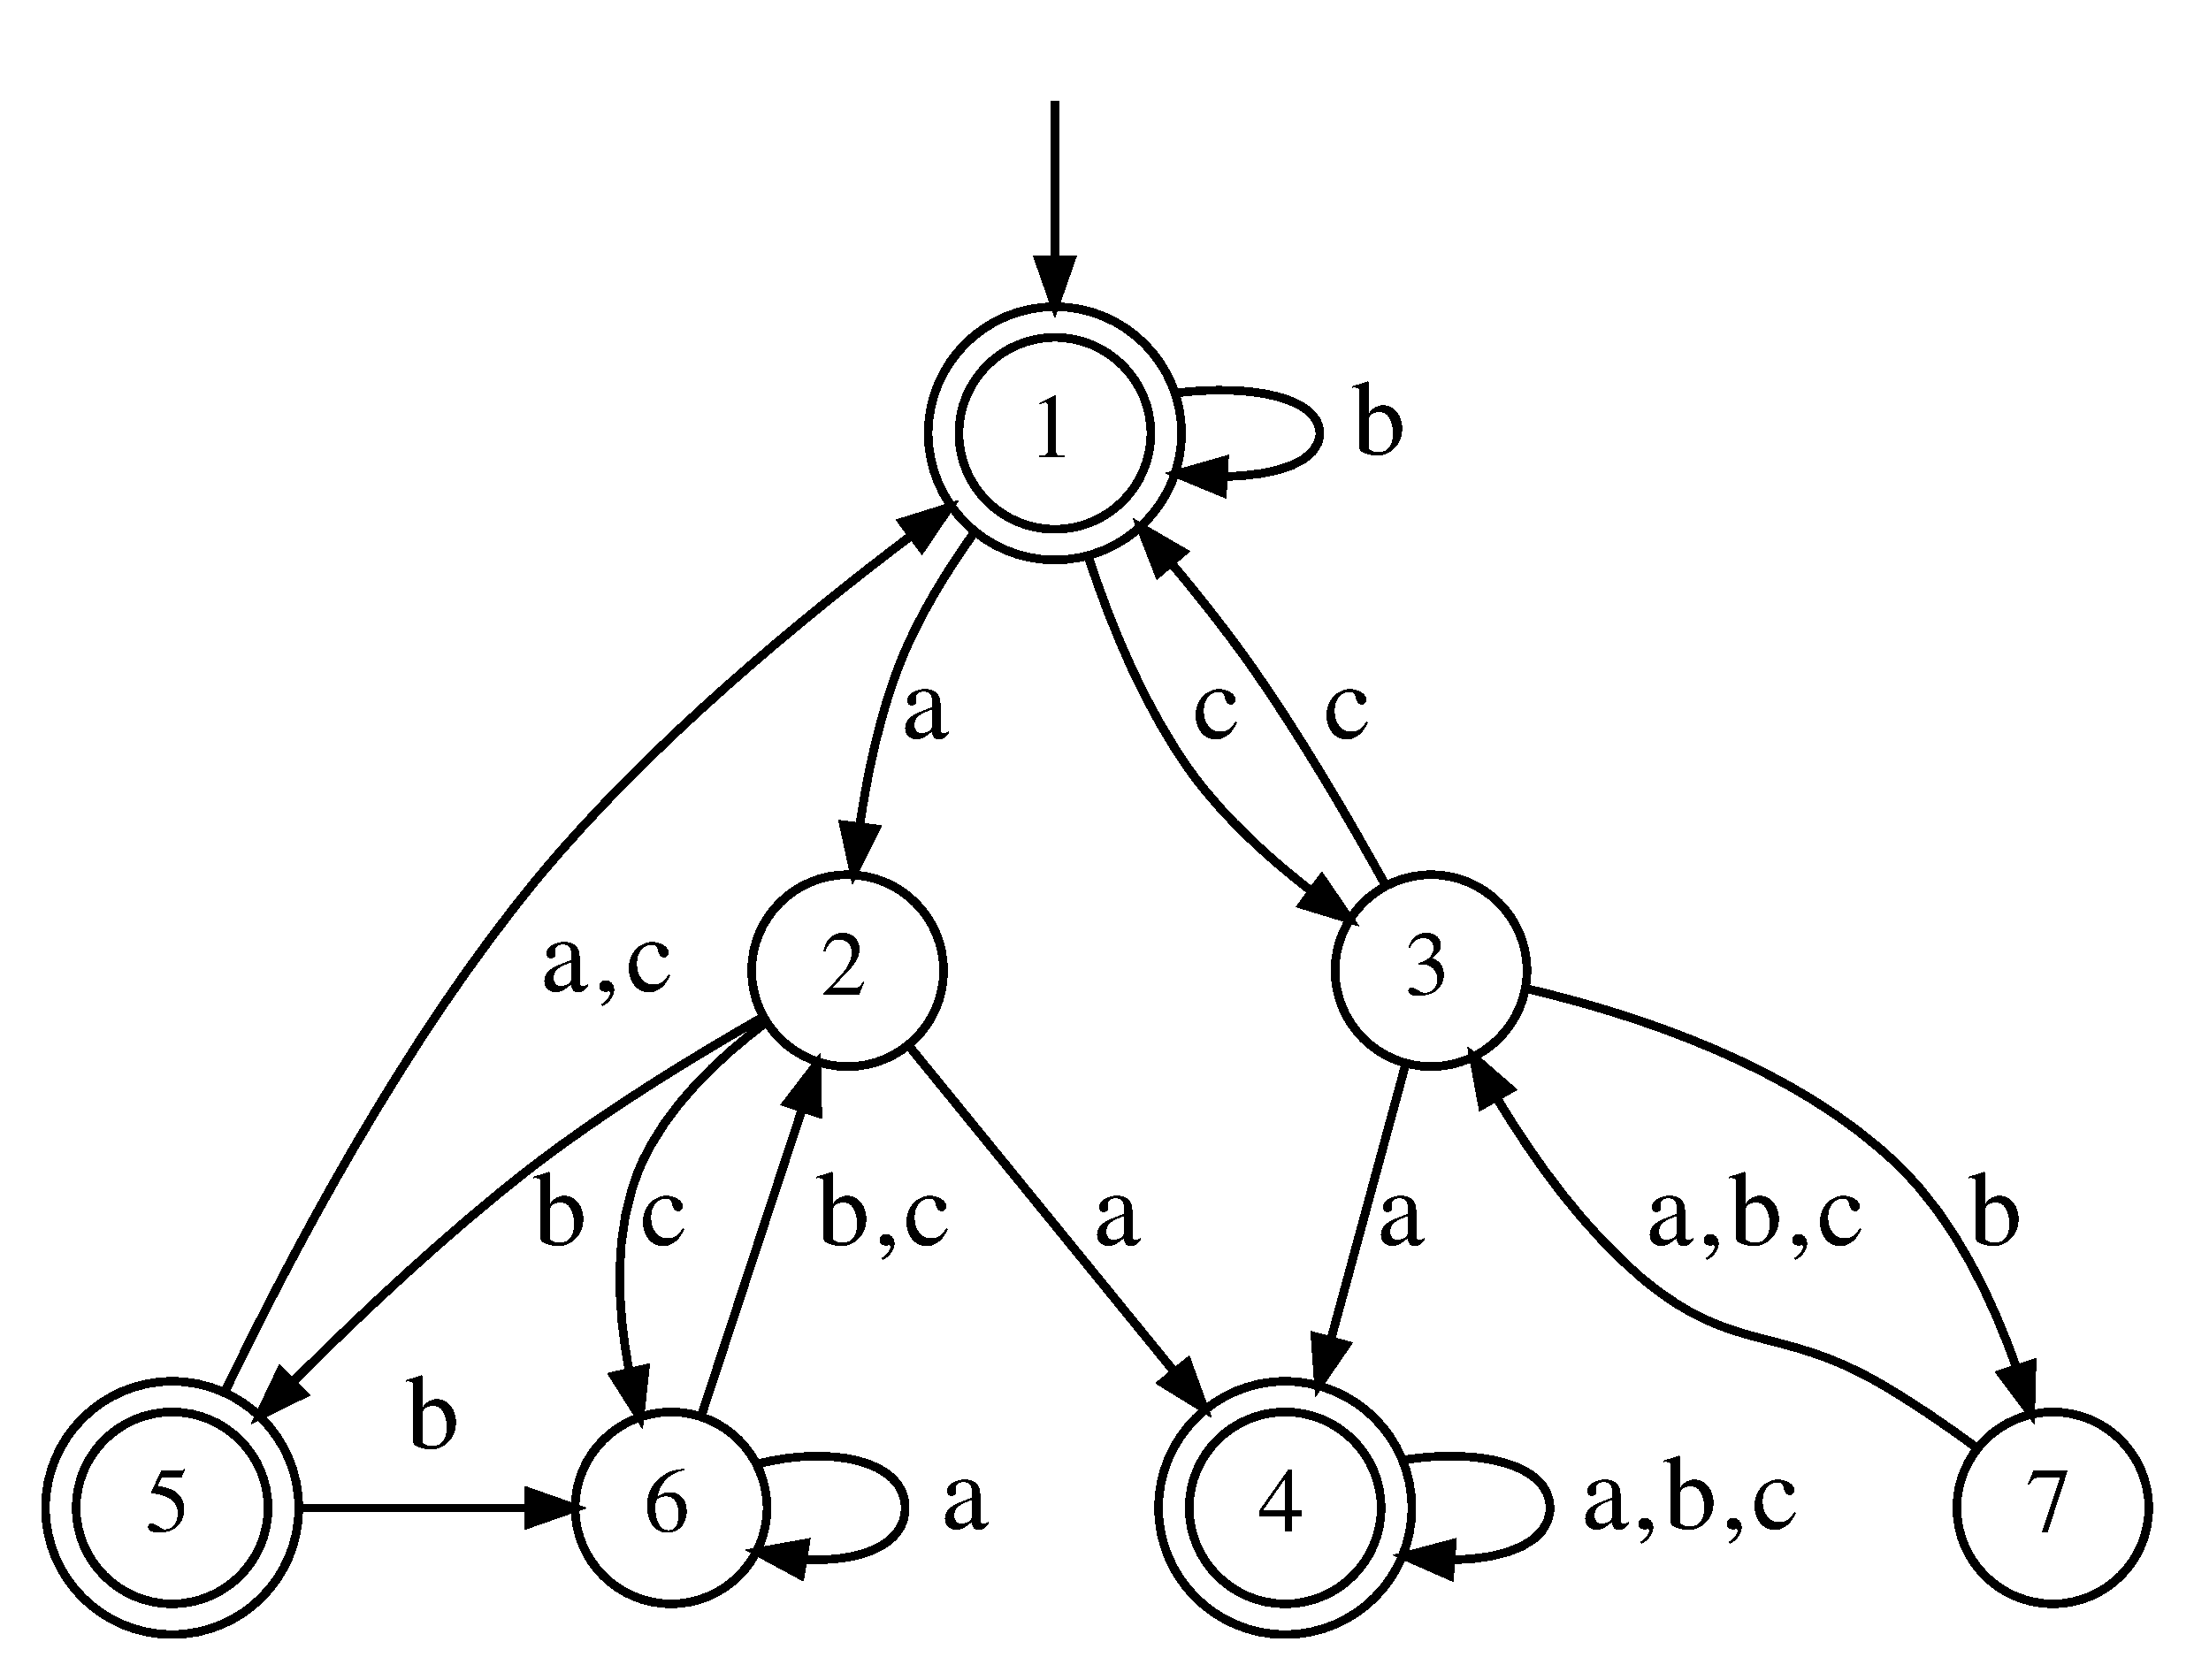
\includegraphics[scale=0.15]{img/datamod/BFS-example.eps}
    \begin{tikzpicture}[
    ->, % makes the edges directed
    >=stealth', % makes the arrow heads bold
    node distance=2.76cm, % specifies the minimum distance between two nodes. Change if necessary.
    every state/.style={thick, fill=gray!10, minimum size = 0pt}, % sets the properties for each ’state’ node
    initial text=$ $, % sets the text that appears on the start arrow
    double distance between line centers=2pt
]
    \node[state, initial above, accepting] (q1) {$1$};
    \node[state] (q2) [below left of=q1, xshift=0.8cm] {$2$};
    \node[state] (q3) [below right of=q1] {$3$};
    \node[state, accepting] (q5) [below left of=q2] {$5$};
    \node[state] (q6) [below of=q2] {$6$};
    \node[state, accepting] (q4) [below right of=q2] {$4$};
    \node[state] (q7) [below right of=q3] {$7$};

    \path 
        (q1) edge [left] node {a} (q2)
        (q1) edge [loop right] node {b} (q1)
        (q1) edge [bend right=10, left] node {c} (q3)
        (q3) edge [bend right=10, right] node {c} (q1)
        (q5) edge [bend left=30, left] node {a,c} (q1)
        (q2) edge [above] node {b} (q5)
        (q2) edge [bend right=10, left] node {c} (q6)
        (q6) edge [bend right=10, right] node [xshift=-1pt] {b,c} (q2)
        (q2) edge [above] node {a} (q4)
        (q3) edge [left] node {a} (q4)
        (q3) edge [bend right=10, left] node {b} (q7)
        (q7) edge [bend right=10, right] node {a,b,c} (q3)
        (q5) edge [above] node {b} (q6)
        (q6) edge [loop below] node {a} (q6)
        (q4) edge [loop below] node {a,b,c} (q4)
        ;
\end{tikzpicture}
  \else
    \begin{tikzpicture}[
    ->, % makes the edges directed
    >=stealth', % makes the arrow heads bold
    node distance=2.1cm, % specifies the minimum distance between two nodes. Change if necessary.
    every state/.style={thick, fill=gray!10, minimum size = 0pt}, % sets the properties for each ’state’ node
    initial text=$ $, % sets the text that appears on the start arrow
]
    \node[state, initial above, accepting] (q1) {$1$};
    \node[state] (q2) [below left of=q1, xshift=0.8cm] {$2$};
    \node[state] (q3) [below right of=q1] {$3$};
    \node[state, accepting] (q5) [below left of=q2] {$5$};
    \node[state] (q6) [below of=q2] {$6$};
    \node[state, accepting] (q4) [below right of=q2] {$4$};
    \node[state] (q7) [below right of=q3] {$7$};

    \path 
        (q1) edge [left] node {a} (q2)
        (q1) edge [loop right] node {b} (q1)
        (q1) edge [bend right=10, left] node {c} (q3)
        (q3) edge [bend right=10, right] node {c} (q1)
        (q5) edge [bend left=30, left] node {a,c} (q1)
        (q2) edge [above] node {b} (q5)
        (q2) edge [bend right=10, left] node {c} (q6)
        (q6) edge [bend right=10, right] node [xshift=-1pt] {b,c} (q2)
        (q2) edge [above] node {a} (q4)
        (q3) edge [left] node {a} (q4)
        (q3) edge [bend right=10, left] node {b} (q7)
        (q7) edge [bend right=10, right] node {a,b,c} (q3)
        (q5) edge [above] node {b} (q6)
        (q6) edge [loop below] node {a} (q6)
        (q4) edge [loop below] node {a,b,c} (q4)
        ;
\end{tikzpicture}
  \fi
  \caption{Пример BFS-пронумерованного автомата}
  \label{img:bfs-ex}
\end{figure}

\begin{figure}[ht]
  \centering
  \ifafour
  % 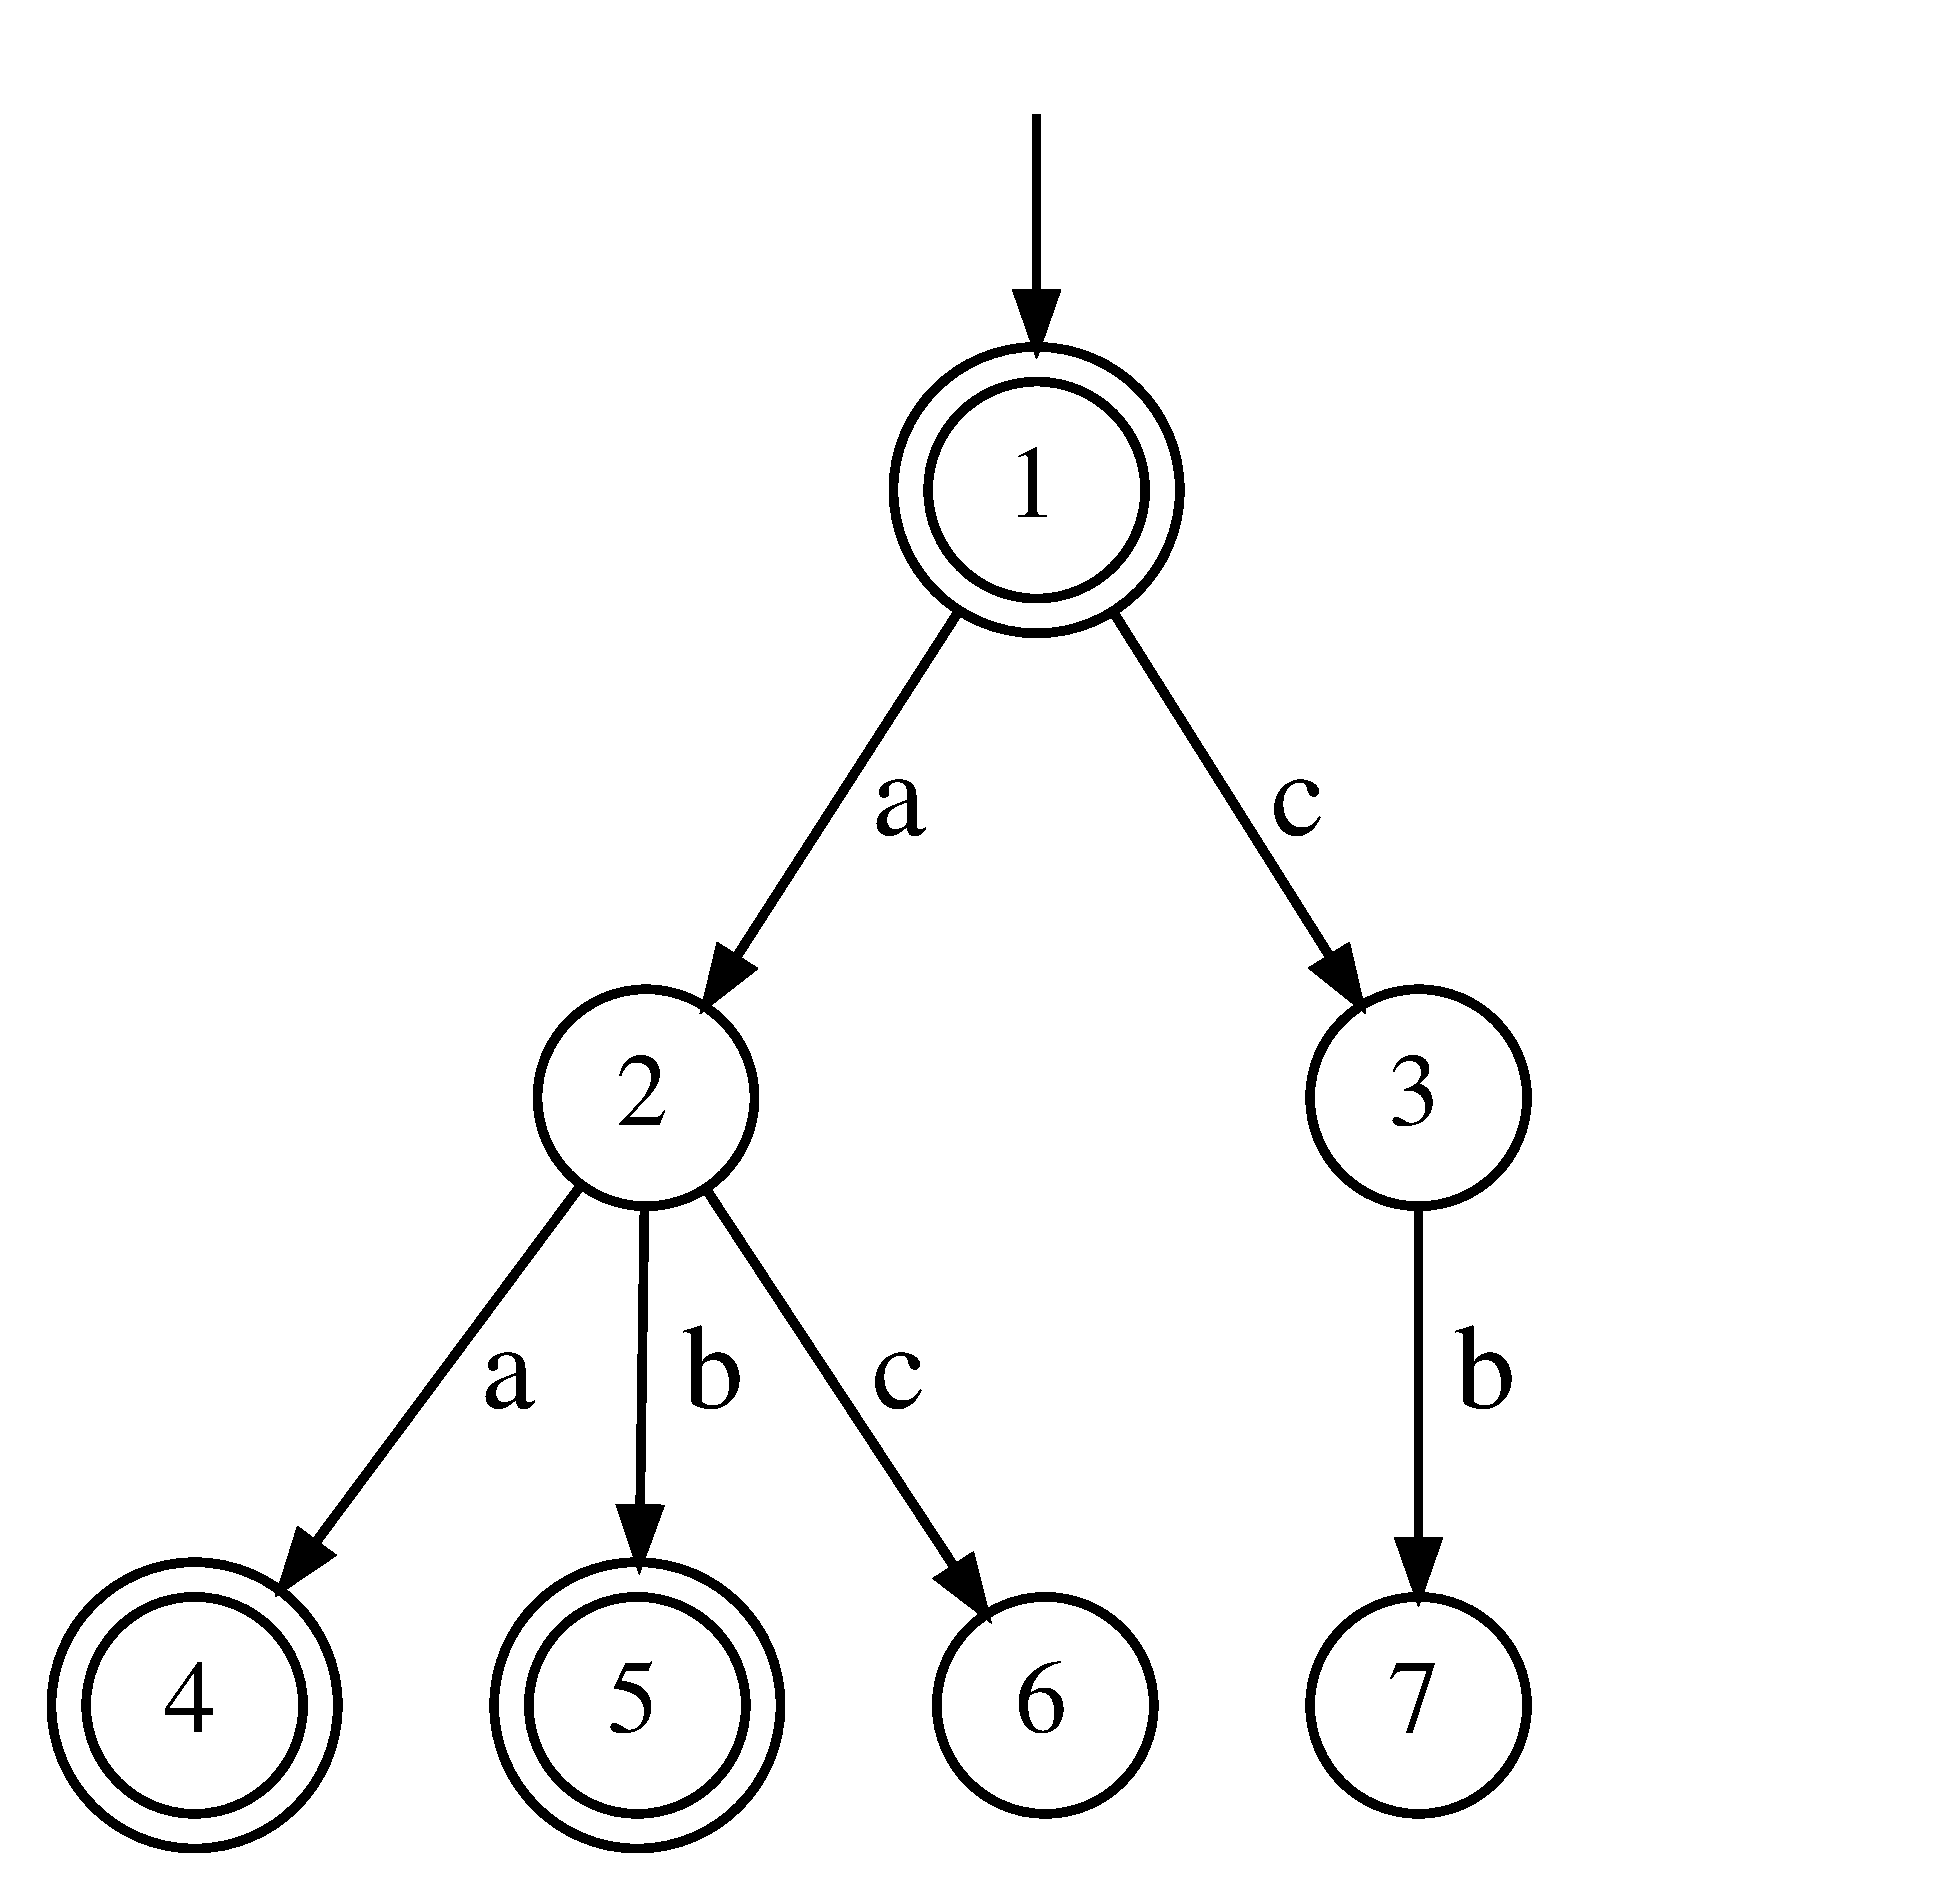
\includegraphics[scale=0.15]{img/datamod/BFS-tree.eps}
    \begin{tikzpicture}[
    ->, % makes the edges directed
    >=stealth', % makes the arrow heads bold
    node distance=2.23cm, % specifies the minimum distance between two nodes. Change if necessary.
    every state/.style={thick, fill=gray!10, minimum size = 0pt}, % sets the properties for each ’state’ node
    initial text=$ $, % sets the text that appears on the start arrow
    double distance between line centers=2pt
]
    \def\xshift{0.53cm}

    \node[state, initial above, accepting] (q1) {$1$};
    \node[state] (q2) [below left of=q1] {$2$};
    \node[state] (q3) [below right of=q1] {$3$};
    \node[state, accepting] (q5) [below of=q2]  {$5$};
    \node[state, accepting] (q4) [left of=q5, xshift=\xshift]  {$4$};
    \node[state] (q6) [right of=q5, xshift=-\xshift]  {$6$};
    \node[state] (q7) [below of=q3]  {$7$};

    \path
        (q1) edge [left] node {a} (q2)
        (q1) edge [right] node {c} (q3)
        (q2) edge [left] node {a} (q4)
        (q2) edge [left] node {b} (q5)
        (q2) edge [right] node {c} (q6)
        (q3) edge [right] node {b} (q7)
        ;
\end{tikzpicture}
  \else
    \begin{tikzpicture}[
    ->, % makes the edges directed
    >=stealth', % makes the arrow heads bold
    node distance=1.7cm, % specifies the minimum distance between two nodes. Change if necessary.
    every state/.style={thick, fill=gray!10, minimum size = 0pt}, % sets the properties for each ’state’ node
    initial text=$ $, % sets the text that appears on the start arrow
]
    \def\xshift{0.53cm}

    \node[state, initial above, accepting] (q1) {$1$};
    \node[state] (q2) [below left of=q1] {$2$};
    \node[state] (q3) [below right of=q1] {$3$};
    \node[state, accepting] (q5) [below of=q2]  {$5$};
    \node[state, accepting] (q4) [left of=q5, xshift=\xshift]  {$4$};
    \node[state] (q6) [right of=q5, xshift=-\xshift]  {$6$};
    \node[state] (q7) [below of=q3]  {$7$};

    \path
        (q1) edge [left] node {a} (q2)
        (q1) edge [right] node {c} (q3)
        (q2) edge [left] node {a} (q4)
        (q2) edge [left] node {b} (q5)
        (q2) edge [right] node {c} (q6)
        (q3) edge [right] node {b} (q7)
        ;
\end{tikzpicture}
  \fi
  \caption{BFS-дерево для автомата, представленного на рисунке~\ref{img:bfs-ex}}
  \label{img:bfs-tree-ex}
\end{figure}

Если закодировать требование к автомату, чтобы он был BFS-пронумерованным, в виде булевых предикатов и добавить к имеющейся формуле, предложенной в~\cite{heule-icgi10}, то программное средство для решения SAT будет искать автоматы, удовлетворяющие заданным примерам поведения, пронумерованные в порядке BFS.
Для того, чтобы закодировать данное требование, было предложено ввести три новых типа булевых переменных:

\begin{enumerate}
  \item переменные родителей $\{p_{j,i}\}_{1 \leq i < j \leq M}$, которые истинны тогда и только тогда, когда состояние $d_i$ является родителем состояния $d_j$ в BFS-дереве автомата $\mathcal{D}$;
  \item переменные наличия переходов $\{t_{i,j}\}_{1 \leq i < j \leq M}$, которые истинны тогда и только тогда, когда в автомате $\mathcal{D}$ существует переход из состояния $d_{i}$ в состояние $d_{j}$;
  \item переменные минимального символа $\{m_{i,l,j}\}_{1 \leq i < j \leq M;l \in \Sigma}$, которые истинны тогда и только тогда, когда в автомате $\mathcal{D}$ из состояния $d_{i}$ в состояние $d_{j}$ существует переход по символу $l$, но не существует переходов по меньшим (согласно выбранному порядку на символах) символам.
  Данные переменные используются только в случае небинарного алфавита.
\end{enumerate}

Используя данные переменные, можно закодировать свойство BFS-пронумерованности автомата с помощью следующих множеств дизъюнктов.

\begin{enumerate}
  \item $\left(t_{i,j} \leftrightarrow y_{i,l_{1},j} \vee y_{i,l_{2},j} \vee \ldots \vee y_{i,l_{L},j} \right)$ для $1 \leq i < j \leq M; l_{k} \in \Sigma$~--- в автомате $\mathcal{D}$ переход из состояния $d_{i}$ в состояние $d_{j}$ существует тогда и только тогда, когду существует переход из состояния $d_{i}$ в состояние $d_{j}$ хотя бы по одному из символов алфавита $\Sigma$.
  
  \item $\left(p_{j,i} \leftrightarrow t_{i,j} \wedge \neg t_{i - 1,j} \wedge \neg t_{i - 2, j} \wedge \ldots \wedge \neg t_{1,j}\right)$ для $1 \leq i < j \leq M$~{---} состояние $d_{i}$ автомата $\mathcal{D}$ является родителем состояния $d_{j}$ в BFS-дереве, если из состояния $d_{i}$ существует переход в состояние $d_{j}$, а из состояний с меньшим номером такого перехода не существует.
  
  \item $\left(p_{j,1} \vee p_{j,2} \vee \ldots \vee p_{j,j - 1}\right)$ для $2 \leq j \leq M$~{---} у каждого состояния $d_{j}$ автомата $\mathcal{D}$, кроме стартового, родитель в BFS-дереве должен иметь меньший номер. 
  Данные дизъюнкты позволяют закодировать порядок по глубине в поддереве.

  \item $\left(p_{j,i} \rightarrow \neg p_{j + 1, k}\right)$ для $1 \leq k < i < j \leq M$~{---} если состояние $d_{i}$ является родителем в дереве BFS состояния $d_{j}$, то у состояния с б\emph{о}льшим номером $d_{j + 1}$ родитель не может иметь номер меньший, чем $i$. 
  Данные дизъюнкты позволяют задать порядок по уровню для детей различных родителей, а также порядок по глубине в разных поддеревьях.
  
  \item $\left(p_{j,i} \wedge p_{j + 1, i} \rightarrow y_{i,l_{1},j}\right)$ для $1 \leq i < j \leq M;\Sigma=\{l_{1},l_{2}\}$~{---} если состояние $d_i$ является родителем в дереве BFS двух состояний $d_{j}$ и $d_{j+1}$ и алфавит бинарный, то переход из состояния $d_{i}$ в $d_{j}$ должен быть по меньшему символу.
  В случае бинарного алфавита данного множества дизъюнктов достаточно, чтобы упорядочить двух детей $d_{j}$ и $d_{j + 1}$ одного состояния $d_{i}$. 
  Дополнительно, для сокращения пространства поиска, можно добавить множество дизъюнктов $\left(p_{j,i} \wedge p_{j + 1, i} \rightarrow y_{i,l_{2},j + 1}\right)$ для $1 \leq i < j \leq M$. 
  Данные дизъюнкты задают порядок по уровню для детей одного родителя в случае бинарного алфавита.

  \item $\left(m_{i,l_{n},j} \leftrightarrow y_{i,l_{n},j} \wedge \neg y_{i,l_{n - 1}, j} \wedge \neg y_{i,l_{n - 2}, j} \wedge \ldots \wedge \neg y_{i,l_{1},j} \right)$ для $1 \leq i < j \leq M; 1 \leq n \leq L;l_{n} \in \Sigma$~{---} в автомате $\mathcal{D}$ символ $l_{n}$ является минимальным символом на переходах из состояния $d_{i}$ в состояние $d_{j}$ тогда и только тогда, когда в автомате существует переход из состояния $d_{i}$ в состояние $d_{j}$ по символу $l_{n}$, но не существует переходов по меньшим (относительно выбранного порядка) символам.
  Данное множество дизъюнктов используется в случае небинарного алфавита.

  \item $\left(p_{j,i} \wedge p_{j + 1, i} \wedge m_{i,l_{n}, j} \rightarrow \neg m_{i, l_{k}, j + 1}\right)$ для $1 \leq i < j \leq M; 1 \leq k < n \leq L;l_n,l_k \in \Sigma$~{---} если состояние $d_{i}$ является родителем в дереве BFS двух состояний $d_{j}$ и $d_{j + 1}$ и алфавит состоит из более чем двух символов, то из состояния $d_{i}$ переход в состояние $d_{j}$ должен быть по меньшему (относительно выбранного порядка) символу чем в состояние $d_{j + 1}$.
  Данные дизъюнкты задают порядок по уровню для детей одного родителя в случае небинарного алфавита.
\end{enumerate}

Все представленные выше наборы дизъюнктов могут быть объединены с помощью конкатенации в одну большую булеву формулу. Всего в такой формуле будет $\mathcal{O}(M^{3} + M^{2} \times L^{2})$ дизъюнктов и для их кодирования будет использовано $\mathcal{O}(M^2 \times L)$ переменных.

%----------------------------------------------------------------------------------------

\section{Подход уточнения абстракции по контрпримерам}
\label{sec:review:cegar}

Программные системы с каждым годом становятся все сложнее, и все сильнее растет их роль в жизни общества~--- все больше различных ответственных промышленных и повседневных процессов автоматизируются с помощью компьютеров и программных средства.
Наличие ошибок в программном коде во многих случаях может привести к серьезным последствиям~\cite{DBLP:journals/ieeesp/ZhivichC09}: значительным финансовым убыткам, утечке важной информации, нанесению вреда здоровью людей и даже к их смерти.
Поэтому значительную актуальность в последние десятилетия приобрела разработка применимых на практике методов проверки корректности программ.
Такие методы можно разделить на две большие группы: динамические и статические методы проверки.
В основе динамических методов лежит методология тестирования, когда проверка за корректностью программы происходит во время ее работы.
Однако, с помощью такого тестирования можно обнаружить только те ошибки, которые проявляются во время конкретного воспроизведенного сценария выполнения программы.
Даже в не самых больших и важных программах зачастую существует такое множество ситуаций, потенциально приводящих к ошибкам, что их полное покрытие тестами не представляется возможным.
Статические же методы проверяют корректность программного кода без его выполнения и запуска программы и потенциально способны обнаружить все возможные ошибки или доказать их отсутствие.
Однако, Тьюринг в 1936 году доказал, что проблема останова неразрешима~\cite{turing1936computable}, и, тем самым, показал, что невозможность существования алгоритма, способного доказать корректность некоторой программы в общем случае.
Впоследствии было предложено множество алгоритмов, способных формально доказывать корректность либо небольших программ, либо каких упрощенных моделей программ.

Среди таких статических методов можно выделить метод \emph{уточнения абстракции по контрпримерам} (counterexample-guided abstraction refinement~--- CEGAR), который впервые был предложен в 2000 году Эдмундом Кларком и коллегами~\cite{DBLP:conf/cav/ClarkeGJLV00}.
Данный метод был разработан для автоматизированного итеративного построения абстрактной модели программы, которую необходимо верифицировать~--- доказать корректность.
Подробный обзор метода уточнения абстракции по контрпримерам можно найти в работе российских ученых Мандрыкина, Мутилина и Хорошилова из Института системного программирования им.~В.П. Иванникова РАН~\cite{мандрыкин2013введение}.

В основе данного метода лежит понятие \emph{абстракции}.
При использовании абстракции вместо реальных состояний верифицируемой программы рассматриваются абстрактные состояния, которые объединяют в себе множества реальных состояний.
При этом, эти множества не обязательно должны быть непересекающимися.
На первом шаге алгоритма выбираются какие-то абстрактные состояния (эвристически, случайно или на основе каких-то известных данных).
Затем, на основе этих состояний строится \emph{абстрактное дерево достижимости}, в котором абстрактные состояния соединены переходом тогда и только тогда, когда переходом соединены какие-то из соответствующих реальных состояний.
Таким образом по построению получается, что все пути, по которым возможно выполнение в реальной программе, также представлены в абстрактном дереве, но не наоборот.

Из вышесказанного следует, что если ошибочные состояния (описывающие нежелательное состояние программы) не достижимы в абстрактном дереве, то они не достижимы и в исходной программе.
Если же существует путь в абстрактном дереве в некоторое ошибочное состояние, то такой путь называется контрпримером.
Наличие контрпримера говорит либо о том, что в исходной программе есть ошибка, либо о том, что построенная абстрактная модель неточна.
Найденный контрпример проверяется на исходной программе и, если соответствующий путь содержится в ней, то в программе найдена ошибка.
Иначе, с помощью найденного контрпримера абстракция уточняется~--- перестраивается абстрактное дерево достижимости.
Данный процесс повторяется до тех пор, пока не будет найдена ошибка в исходной программе, либо пока не будет доказано, что в исходной программе ошибки отсутствуют.

Несмотря на то, что данный метод скорее относится к классу методов активного обучения, перспективным выглядит применение схожей идеи для улучшения точных методов генерации ДКА по заданны примерам поведения.
Так, всеми методами, основанными на сведении к SAT, генерируется булева формула, размер которой линейно зависит от размера расширенного префиксного дерева~--- $\mathcal{O}\left(N\times M^{2}\right)$, где $N$~--- размер префиксного дерева, а $M$~--- размер генерируемого автомата (см. раздел~\ref{sec:review:sat-dfa-inf:sat}).
Таким образом, при наличии \emph{избыточного} числа примеров поведения и относительно небольшом ДКА, булева формула, кодирующая задачу генерации ДКА, может быть слишком большой для современных программных средств для решения SAT.
В настоящей диссертации будет разработан метод, позволяющий совместить в себе сведение к SAT и идеи подхода уточнения абстракции по контрпримерам, для генерации ДКА.

% %----------------------------------------------------------------------------------------

% \section{Задачи, решаемые в диссертационной работе}
% \label{sec:review:tasks}

% \inote{написать ``как итог'' про недостатки существующих подходов и рассказать про задачи, которые будут решаться в данной работе}

% На основании проведенного обзора были выделены следующие задачи диссертационного исследования.
% \begin{enumerate}
%   \item Разработка предикатов нарушения симметрии, основанных на алгоритмах обхода графа в ширину и в глубину, для сокращения пространства поиска при решении задачи выполнимости.
%   Разработка и реализация точных методов генерации ДКА по заданным примерам поведения, использующих данные предикаты, проведение экспериментальных исследований с ними.

%   \item Разработка и реализация точного метода генерации ДКА по избыточному набору примеров поведения с использованием сведения к задаче выполнимости и подхода уточнения абстракции по контрпримерам.
%   Проведение экспериментальных исследований с методом.
  
%   \item Разработка и реализация метода генерации всех неизоморфных ДКА минимального размера, удовлетворяющих заданным примерам поведения, с использованием предикатов нарушения симметрии и программных средств решения задачи выполнимости.
%   Проведение экспериментальных исследований с методом.
% \end{enumerate}

%----------------------------------------------------------------------------------------

\chresults{\ref{sec:review}}

В первой главе был произведен обзор предметной области, приведена терминология, а также изложены известные результаты ряда разделов информатики, необходимых для описания предлагаемых в диссертации методов:

Дана постановка задачи SAT, приведены необходимые определения, а также описаны основные методы решения данной задачи.
Задача выполнимости является одной из самых активно исследуемых NP-трудных задач, что подтверждается проведением ежегодных конференций, посвященных SAT, а также проведением ежегодных соревнований по выявлению лучшего программного средства для ее решения.
Поэтому множество других задач из класса NP могут быть эффективно решены при помощи сведения к задаче выполнимости и использования современных программных средств для решения SAT.
Однако, несмотря на постоянное повышение эффективности методов решения SAT, в худшем случае для поиска решения требуется экспоненциальное относительно размера входных данных время.

Даны базовые понятия о детерминированных конечных автоматах, об изоморфизме и постановка задачи генерации ДКА по заданным примерам поведения.
Также, приведено определение расширенного префиксного дерева~--- древовидной структуры данных для представления множества примеров поведения.

Проведен анализ работ, посвященных методам генерации ДКА по заданным примерам поведения.
Рассмотрены три различных типа методов генерации ДКА, основанных на: эвристических алгоритмах (различные методы слияния состояний); метаэвристических алгоритмах (генетические и муравьиные алгоритмы); сведении к NP-полным задачам раскраски графа и выполнимости булевой формулы.
Эвристические и метаэвристические методы являются неточными~--- первые не гарантируют минимальности сгенерированного ДКА, вторые вообще не гарантируют, что какой-то автомат будет найден за конечное время.
Методы, основанные на сведении к NP-полным задачам являются точными~--- ими гарантируется, что ДКА, удовлетворяющий примерам поведения, будет найден за конечное время и будет состоять из минимального числа состояний.

Также был описан подход уточнения абстракции по контрпримерам, изначально предложенный для итеративного построения модели программного обеспечения для последующей верификации.

Исходя из анализа литературы можно сделать следующие выводы.
\begin{itemize}
  \item Булева формула, получаемая при генерации ДКА большого размера по большому числу примеров поведения при помощи сведения к SAT, зачастую слишком сложна для современных программных средств для решения SAT, что актуализирует разработку новых предикатов нарушения симметрии, сокращающих пространство поиска.
  
  \item Предложенное ранее кодирование предикатов нарушения симметрии на основе BFS, образуют булеву формулу, состоящую из $\mathcal{O}\left(M^{3} + M^{2} \times L^{2}\right)$ дизъюнктов (где $M$~--- размер генерируемого ДКА, $L$~--- размер алфавита), что неприменимо для автоматов большого размера.
  
  \item Размер булевой формулы зависит от размера расширенного префиксного дерева, а значит и от числа и длины заданных примеров поведения.
  В случае избыточного набора примеров поведения не существует применимых на практике методов генерации ДКА.
  Потенциальным решением может стать разработка метода, сочетающего в себе сведение к задаче выполнимости и идеи подхода уточнения абстракции по контрпримерам.

  \item Ранее не предлагалось методов генерации всех неизоморфных ДКА минимального размера, соответствующих заданным примерам поведения.
  Более того, без использования предикатов нарушения симметрии на основе кодирования алгоритма BFS, разработка эффективных методов генерации всех ДКА не представляется возможной ввиду комбинаторного взрыва числа рассматриваемых автоматов.
\end{itemize}